%\documentclass{article}
\documentclass[onecolumn]{IEEEconf}
%\usepackage{a4wide}
\usepackage{enumitem}
\usepackage[usenames, dvipsnames]{color}
\usepackage{graphicx}
\usepackage{subcaption}
\renewcommand{\figurename}{Fig.}
\renewcommand*{\thetable}{\Roman{table}}
\usepackage[normalem]{ulem}
\usepackage[labelformat=simple]{subcaption}
\renewcommand\thesubfigure{(\alph{subfigure})}
\usepackage{multirow}

\title{Response to the Reviewers' Comments}
\begin{document}

\maketitle


The authors would like to thank the reviewers for the precious comments and suggestions on the technical contents and presentation of our manuscript ``Runtime Power Management of Battery Electric Vehicles for Extended Range with Consideration of Driving Time," submitted to IEEE Transactions on Very Large Scale Integration (TVLSI.) This revised manuscript has been greatly improved thanks to the reviewers' invaluable advices. 
We have revised the manuscript faithfully following the reviewers's comments. We include the newly added or significantly modified parts in the revised version of the paper also in Response to Reviewers. We highlight the important technical content changes and set those parts in a red color in the revised paper. 

All the modified sentences in the revised manuscript are highlighted in Red for better readability. Detailed comments and corresponding corrections are listed below:\\

\setlength{\parindent}{0cm}
%%%%%%%%%%%%%%%%%%%%%%%%%%%%
\textbf{[REVIEWER 1]}
%%%%%%%%%%%%%%%%%%%%%%%%%%%%
\begin{description}
\item [R1-C1] The structure of introduction should be improved. First, it is interesting to mention the difference between ICEV and EV. However, it is not clear why the paper spends a relative paragraph to explain ICEV while the topic of this paper is on EV. Second, it is good to mention the whole structure of this paper.
 
\item [R1-A1] One of the strong motivations of this paper is that we found the previous eco-driving work for ICEV does not work for BEV due to the fundamental discrepancy between the engine powertrain and electric powertrain. Since eco-driving methods for ICEV are not new, we start with the motivational observation how the ICEV powertrain is different from the EV powertrain in Introduction followed by demonstration of the minimum-energy speed versus road slope both for ICEV and EV in Section III. We assume most TVLSI audiences are not very much familiar with ICEV powertrain. Such logic flow is important to clarify novelty of this work. In more detail,  we describe the differences of 1) power consumption models of ICEV and BEV powertrains, 2) power consumption characteristics on various road slopes and 3) the efficiency maps between internal combustion engines and electric motors.  

Nevertheless, we also agree on that such logic flow could be improved as the reviewer raised such a question. So, we add a description that summarizes the paper structure at the end of Introduction reflecting the reviewer's recommendation.

\textcolor{red}{We summarize the paper structure as follows. Section~II describes related work for low-energy driving for both ICEV and EV. Section~III introduces analysis of power consumption of ICEV and EV  by the vehicle setup and driving conditions. This section also compares power consumption characteristics of EV with those of ICEV and demonstrates why  ICEV eco-driving results can hardly apply to EV. Section~IV introduces a framework to derive EV-specific energy-aware-velocity planning. In this section, we are first to introduce new performance metrics and their solution methods to take into account both driving energy and driving time: energy-delay product ($EDP$), energy-square-delay product ($E^2DP$) and energy-cubic-delay product ($E^3DP$). Section V demonstrates the experimental results. 
We also visualize the impacts of the model fidelity on the energy-aware-velocity planning in Section~VI. Section~VII is a summary of major technical contribution of this paper.}\\


\item [R1-C2] It is not clear how to validate the power model of EV. As the author mentions that accuracy of power model is quite important, it is good to see the power model in this paper can be validated by some real measurement results.

\item [R1-A2] Previous eco-driving research is optimized for ICEVs that mandate a (variable-speed) transmission, and thus the resultant eco-driving is not applicable to EVs as we demonstrated in this paper. We previously introduced an accurate EV-specific power model and demonstrated that  EV energy consumption and driving range estimation fidelity is largely affected by the model fidelity [1]. 

In this paper, we use the same EV power model equation in [1], which has been proven to be accurate as long as the coefficients are appropriate. However, the model coefficients in [1] are only for low-speed, ultra light-weighted EV (a half metric Ton). However, we would like to demonstrate a more practical results that are applicable to production EVs. Therefore, all the coefficients should be updated for production-scale EVs in this paper. 

Here goes how we extracted correct coefficients of the EV power equation. We use a vehicle simulator that supports EV as well, ADVISOR, to extract the coefficients of new vehicles starting from known vehicle specifications such as the aerodynamic resistance, rolling resistance, curb weight, and so on. Such data is often published in the users' manual, website and so forth. We further use the vehicle performance data such as the top speed, maximum acceleration, and so on, which are also available on the manuals and website. We iteratively run ADVISOR and derive the model coefficients so that all the known values match among each other. We evaluate the model accuracy with the range-speed real vehicle experiments as shown in Fig. 1(a), which has been published by [32], [33], [34], [35], [36]. We further refine the coefficients until all the available data values match well. Finally, the derived EV power model well matches with the range-speed experimental data as shown in Fig. 1(b) as well as the top speed and maximum acceleration, setting the aerodynamic resistance, rolling resistance, curb weight, etc. with the known (fact) values. The errors of the range-speed simulation is merely 1.4\%, the time to approach 60 mph at departure is 7.8\%, and the top speed is 3.0\%, respectively. \uline{We revised the manuscript adding the following paragraph with a new figure in Section III-A on page 3 and 4.} \\

%%%%%%%%%%%%%%%%%
\textcolor{red}{We use ADVISOR to extract the model coefficients of new vehicles starting from known vehicle specifications such as the aerodynamic resistance, rolling resistance, curb weight, and so on. Such data is often published in the users' manual, website and so forth. We further use the vehicle performance data such as the top speed, maximum acceleration, and so on, which are also available on the manuals, commercials and websites. We iteratively run ADVISOR and derive the model coefficients so that all the known data values match among each other.}
The model coefficient extraction result shows as in Fig.~1. The normalized root-mean-square (RMS) deviation is 5.1\%. Table I summarizes the model coefficients of (5) for Chevrolet Bolt.

\textcolor{red}{We further evaluate the model accuracy with the range-speed real vehicle experiments as shown in Fig.~2(a) to confirm the derived power models are close enough to the real vehicle measurement data~[32], [33], [34], [35], [36]. We  refine the coefficients until all the available data values match well. \\
As a result, the derived EV power model well matches with the range-speed experimental data as shown in Fig.~2(b) as well as the top speed and maximum acceleration setting the aerodynamic resistance, rolling resistance, curb weight, etc. with the known values. The errors in the range-speed simulation is merely 1.4\%, the time for 0-to-100 km/h error is 7.8\%, and the top speed error is 3.0\%, respectively.} 


\begin{figure} [h!]  %Figure 2.
 \renewcommand\thefigure{2}
\centering
	\begin{subfigure}{0.47\textwidth}
	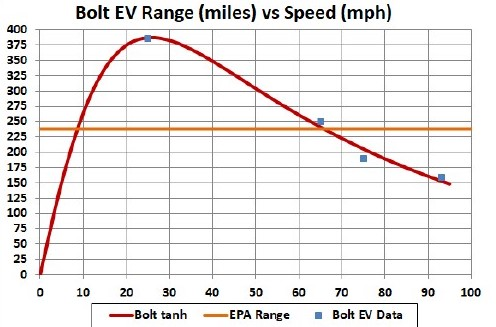
\includegraphics[width=\hsize]{Figures/Bolt_EV_range.jpg}
	\caption{Range-speed experimental data.}
	\label{fig:range_speed_exp}
	\end{subfigure}
%~
	\begin{subfigure}{0.47\textwidth}
	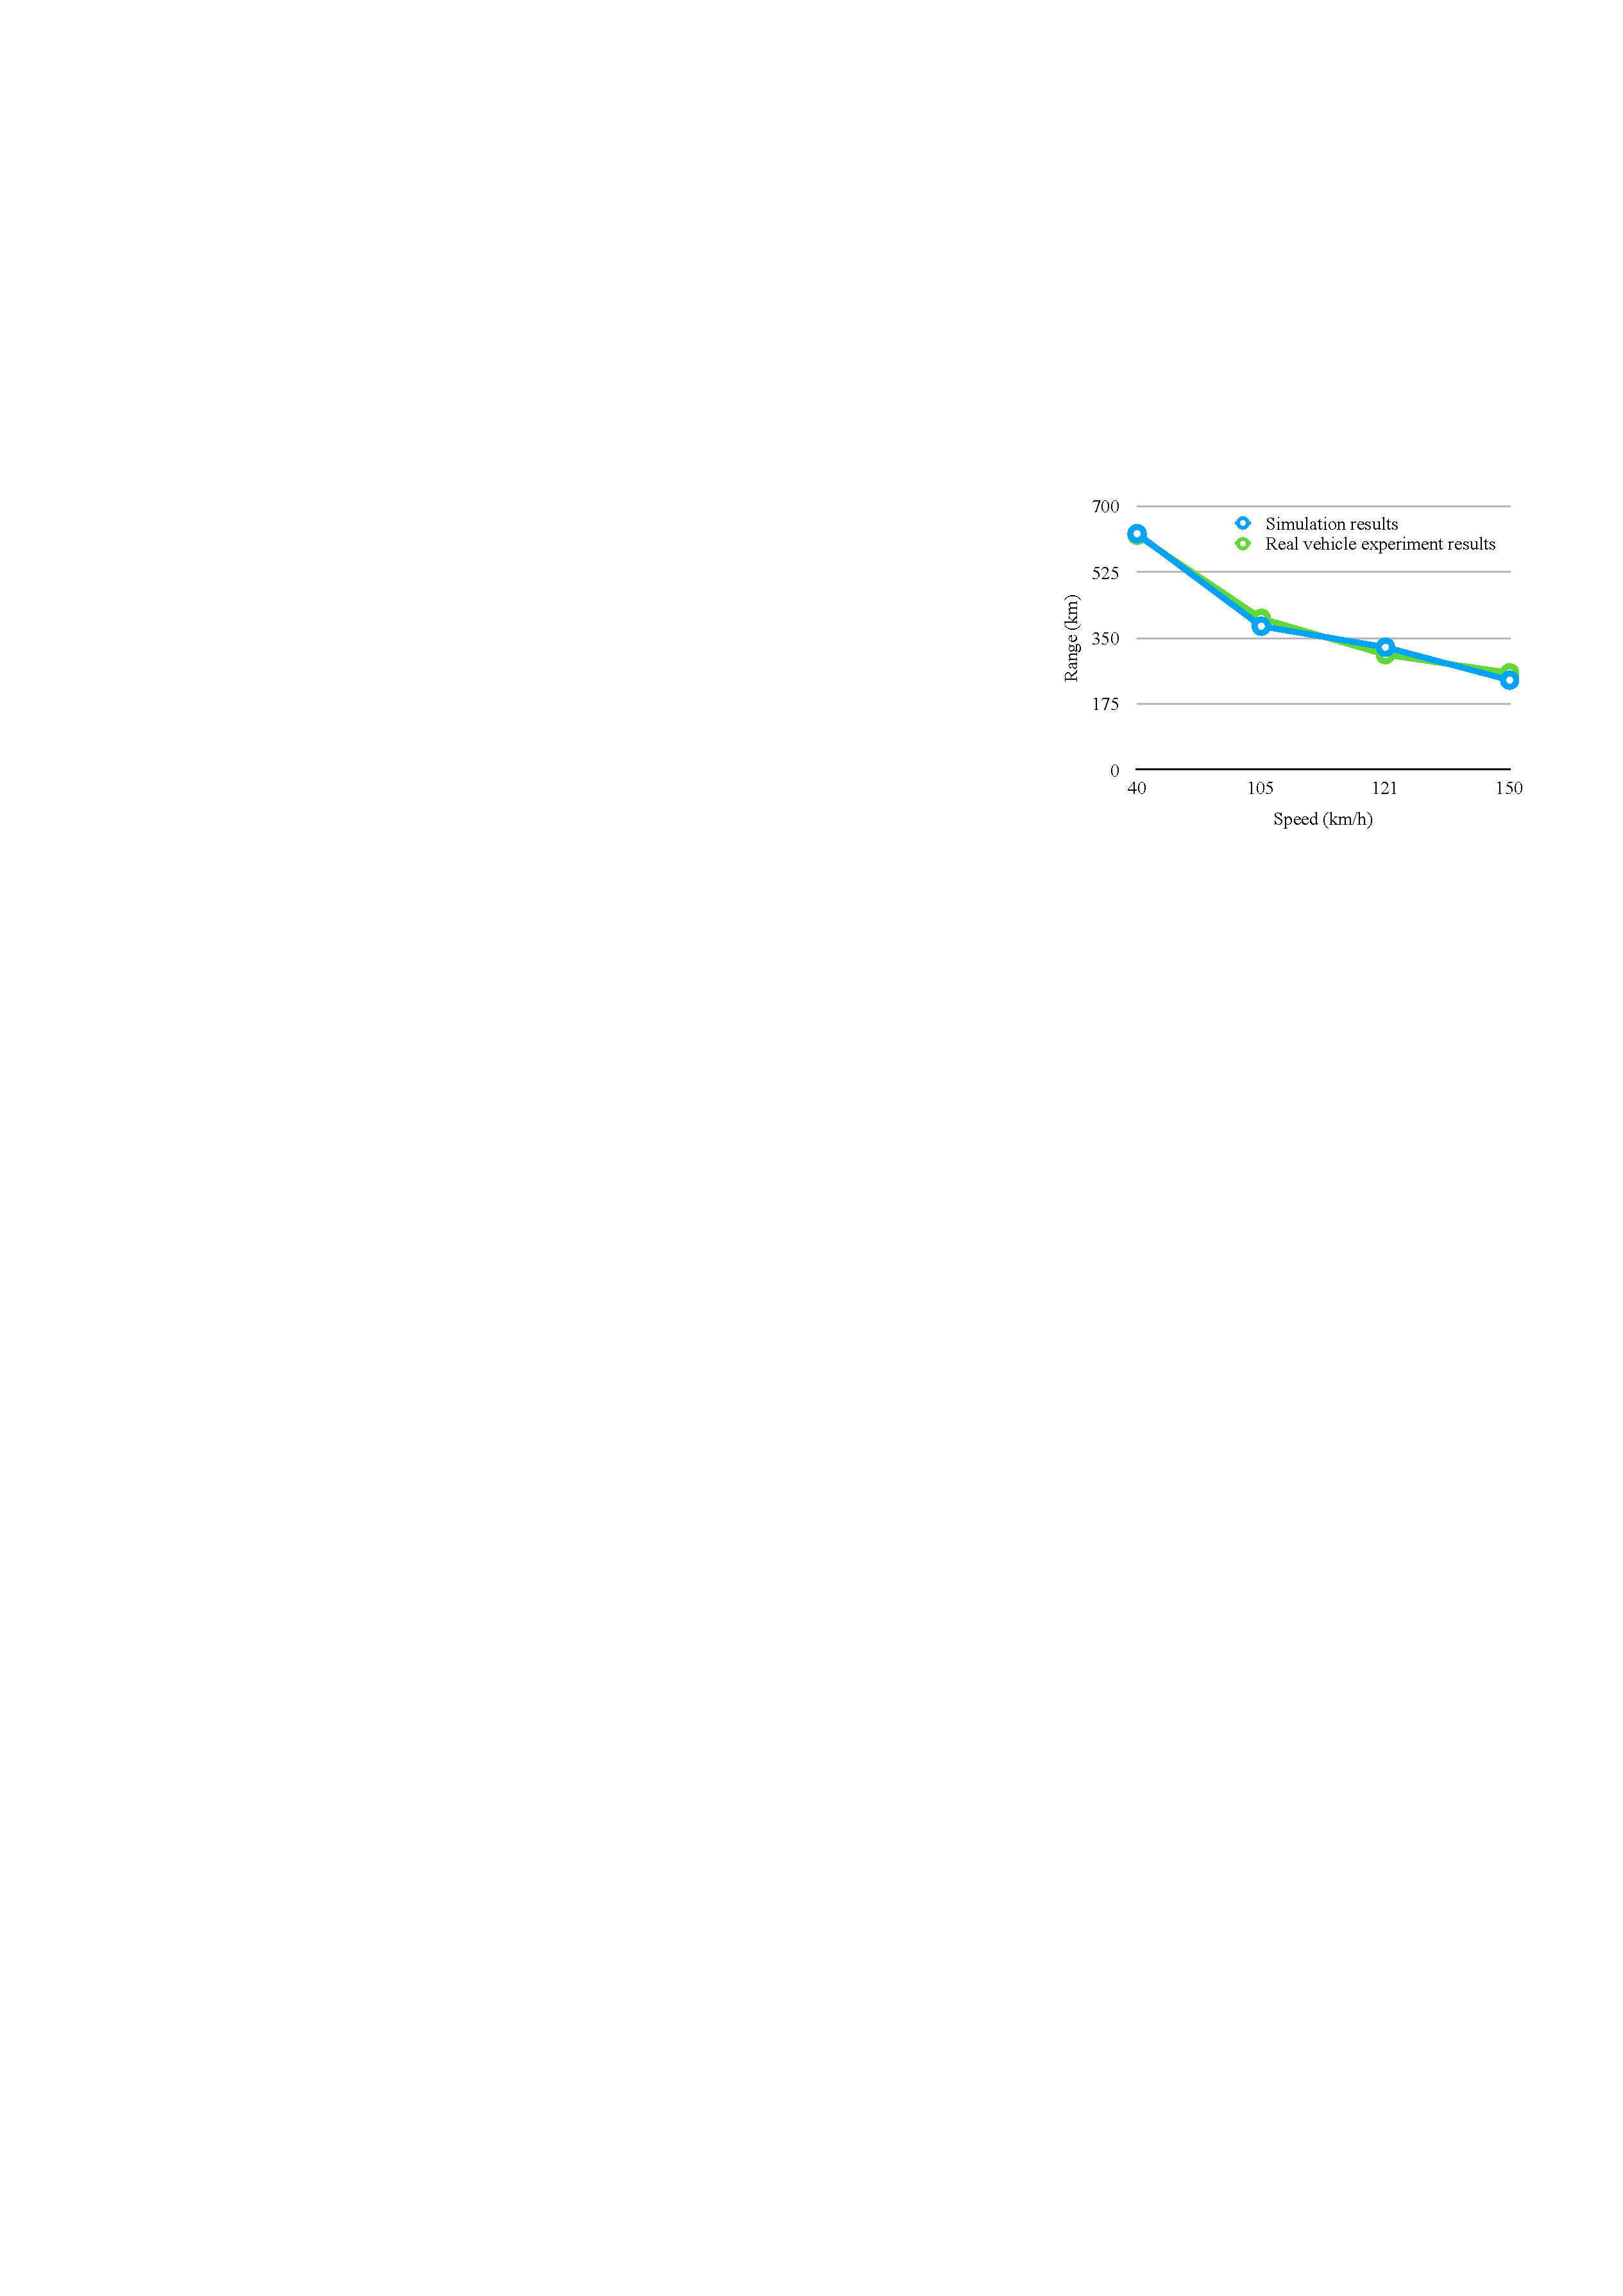
\includegraphics[width=\hsize]{Figures/Range-speed_validation.pdf}
	\caption{Range comparison with simulation results.}
	\label{fig:range_speed_valid}
	\end{subfigure}
\caption{\textcolor{red}{(a) Range-speed experimental data for Chevrolet Bolt~[36] and (b) comparison with simulation results of the proposed EV power model.}}
\end{figure}

We also added a new reference:

[36] ``Chevrolet bolt EV,'' Genealogy Web Page of L. David Roper, http://www.roperld.com/science/chevybolt.htm.

\item [R1-C3] The optimality of the proposed scheduling algorithm is unclear. The author should add several paragraphs to discuss this topic. It is also to see the comparison baseline is well accepted to show the advantage of the proposed algorithm.

\item [R1-A3] As we already mention in the previous version of the manuscript, the proposed EDP-aware-velocity planning is not optimal. This is because the EDP-aware-velocity planning is not formulated as DP (we also mentioned this in the previous version of the manuscript), but we used DP referring it as ``heuristics.'' We demonstrated that such heuristics method still very well reduces $EDP$, $ED^2P$ and $ED^3P$. However, as the reviewer pointed out, there was no tangible clue how the resultant solutions are close to the true optimal.

In this revised manuscript, we did spend an extended period of time and added a new content  how close the proposed heuristics method is to the true optimal, comparing with the results of Genetic algorithm (GA). GA can hardly be used for a practical solution method as its time complexity is not suitable for real applications. We use the GA results as a golden reference to evaluate the optimality of the proposed heuristics.

We divide a given driving route into multiple segments so that the solution of GA indicates a set of velocity values for each segment. We evaluate the GA solutions and choose one of the solutions. We apply the vehicle acceleration and deceleration constraints so that the velocity difference at the boundary of two adjacent segments becomes close enough to avoid a jerky motion. We update the solution through crossover and mutation processes until the solution converges. The proposed EDP-aware-velocity planning is merely 4.3\% higher than the true EDP-minimum-velocity planning on average. Through this results, we confirm that the results of the proposed heuristics are close enough to the true optimal solutions. We include the comparison with GA in the revised version of the manuscript. We revised the associated sentences as follows:\\

\uline{We added the sixth and seventh paragraphs in IV-E on page 8 as follows:}\\
\textcolor{red}{As the proposed solutions for  $EDP$-, $E^2DP$- and $E^3DP$-aware-velocity planning are not optimal, we perform  validation how close the proposed heuristics method is to the true optimal, comparing with the results of GA. We use the GA results as a golden reference to evaluate the optimality of the proposed heuristics.
%GA can hardly be used for a practical solution method as its time complexity is not suitable for real applications. %
We divide a given driving route into multiple segments so that the solution of GA indicates a set of velocity values for each segment. %We evaluate the GA solutions and choose one of the solutions. 
We apply the vehicle acceleration and deceleration constraints so that the velocity difference at the boundary of two adjacent segments becomes close enough to avoid a jerky motion. We update the solution through crossover and mutation processes until the solution converges.} 


\uline{We modified the ninth paragraph in IV-C on page 8 as follows:}\\
Fig.~12 summarizes $EDP$ of the least-energy-constant-velocity driving, the minimum-delay-constant-velocity driving, the minimum-energy-velocity planning, the velocity planning with $EDP$, $E^2DP$ and $E^3DP$ as a metric on the road benchmarks \textcolor{red}{and the minimum-EDP-velocity planning with GA}. The proposed velocity planning results in up to 46.2\% improvements of $EDP$ compared with the least-energy-constant-velocity driving. 
%The improvements occur especially when the slope of the uphill is steep.
The driving velocity on a flat road is faster than that of the least-energy-constant-velocity driving at the expense of relatively little energy to save driving time. Then, the velocity decreases when climbing the following uphill to spend less motor torque, which saves more energy.

\textcolor{red}{In addition, EDP of the proposed EDP-aware-velocity planning is merely 4.3\% higher than that of the true EDP-minimum-velocity planning on average. Through this results, we confirm that the results of the proposed heuristics are close enough to the true optimal solutions.}\\

We also updated Fig. 12 and Fig. 13:

\begin{figure}
\centering
\renewcommand\thefigure{12}
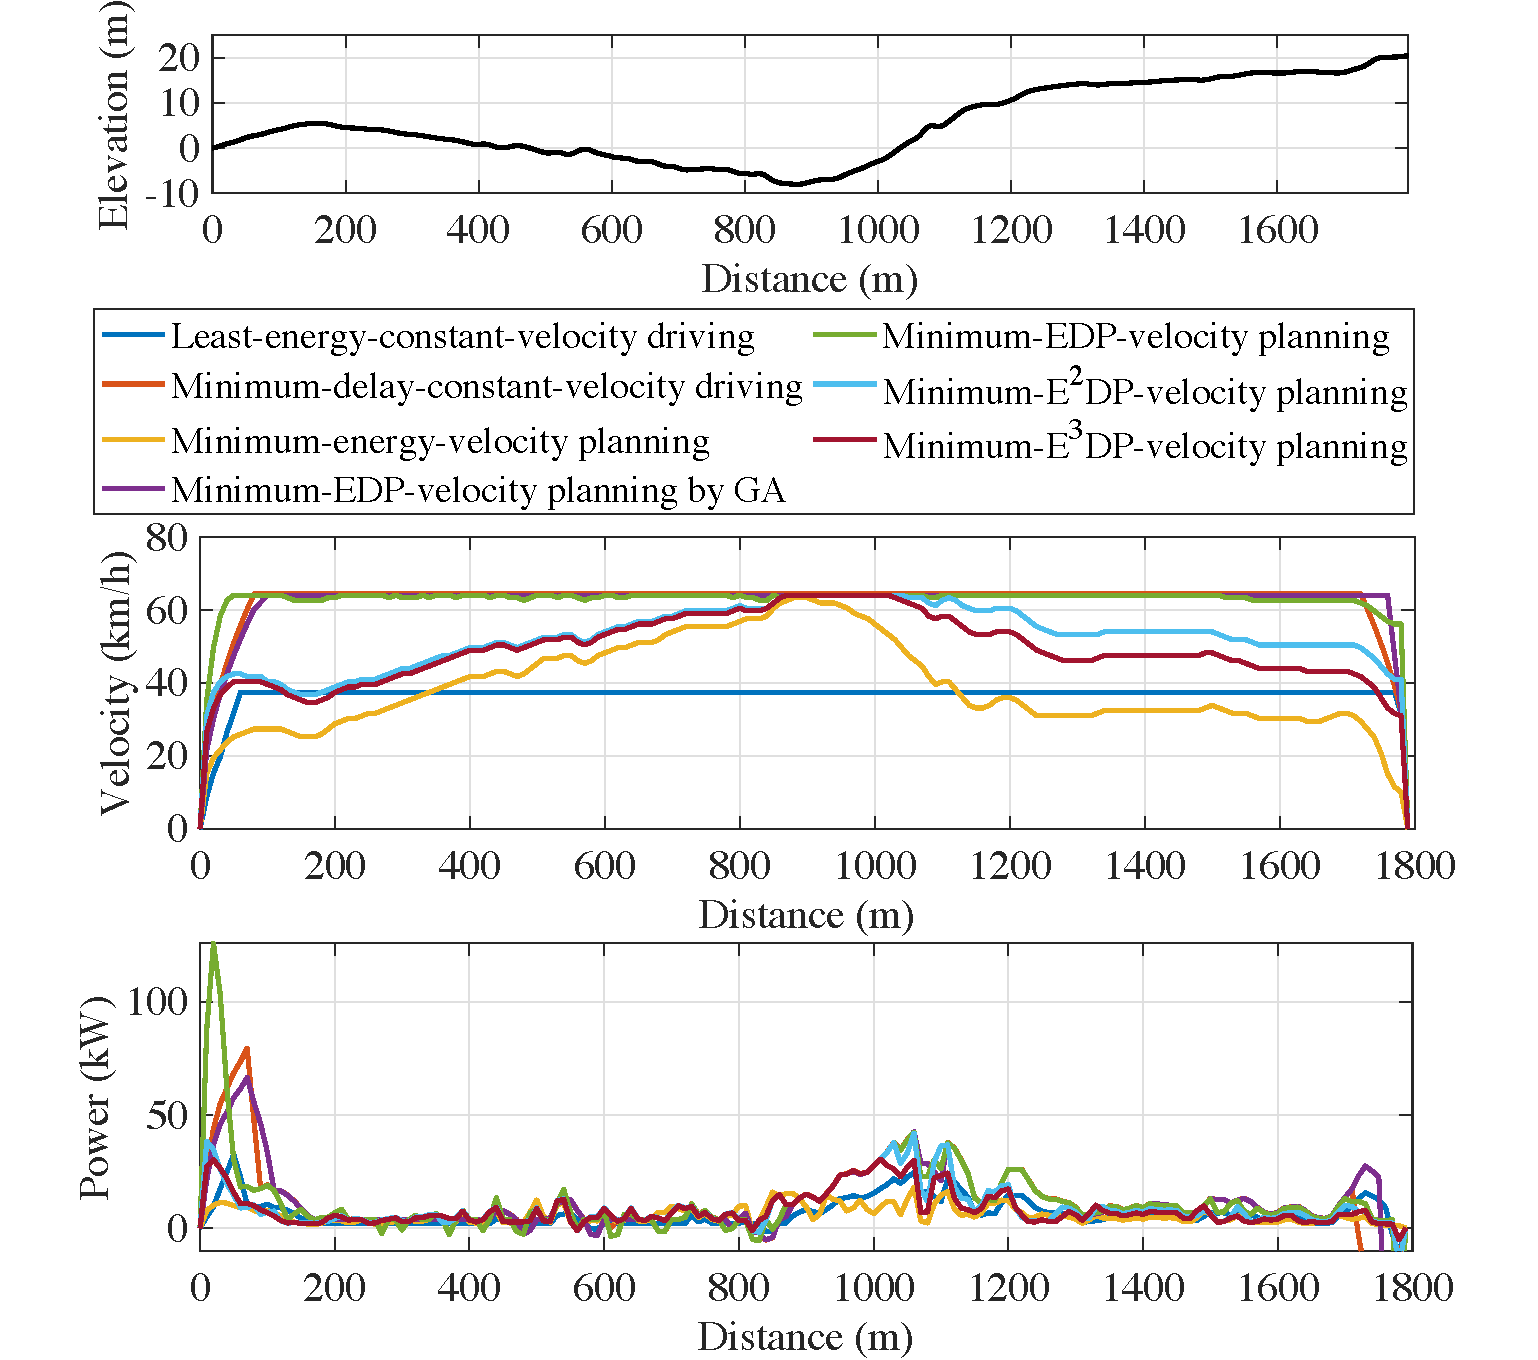
\includegraphics[width=0.6\hsize]{Figures/EDP_comp_profile.pdf}
\caption{\textcolor{red}{Velocity profile comparison with $EDP$, $E^2DP$ and $E^3DP$ on  Serrano Avenue in Anaheim Hills.}}
\label{fig:EDP_aware_velocity_planning}
\end{figure} 

\begin{figure}
\centering
\renewcommand\thefigure{13}
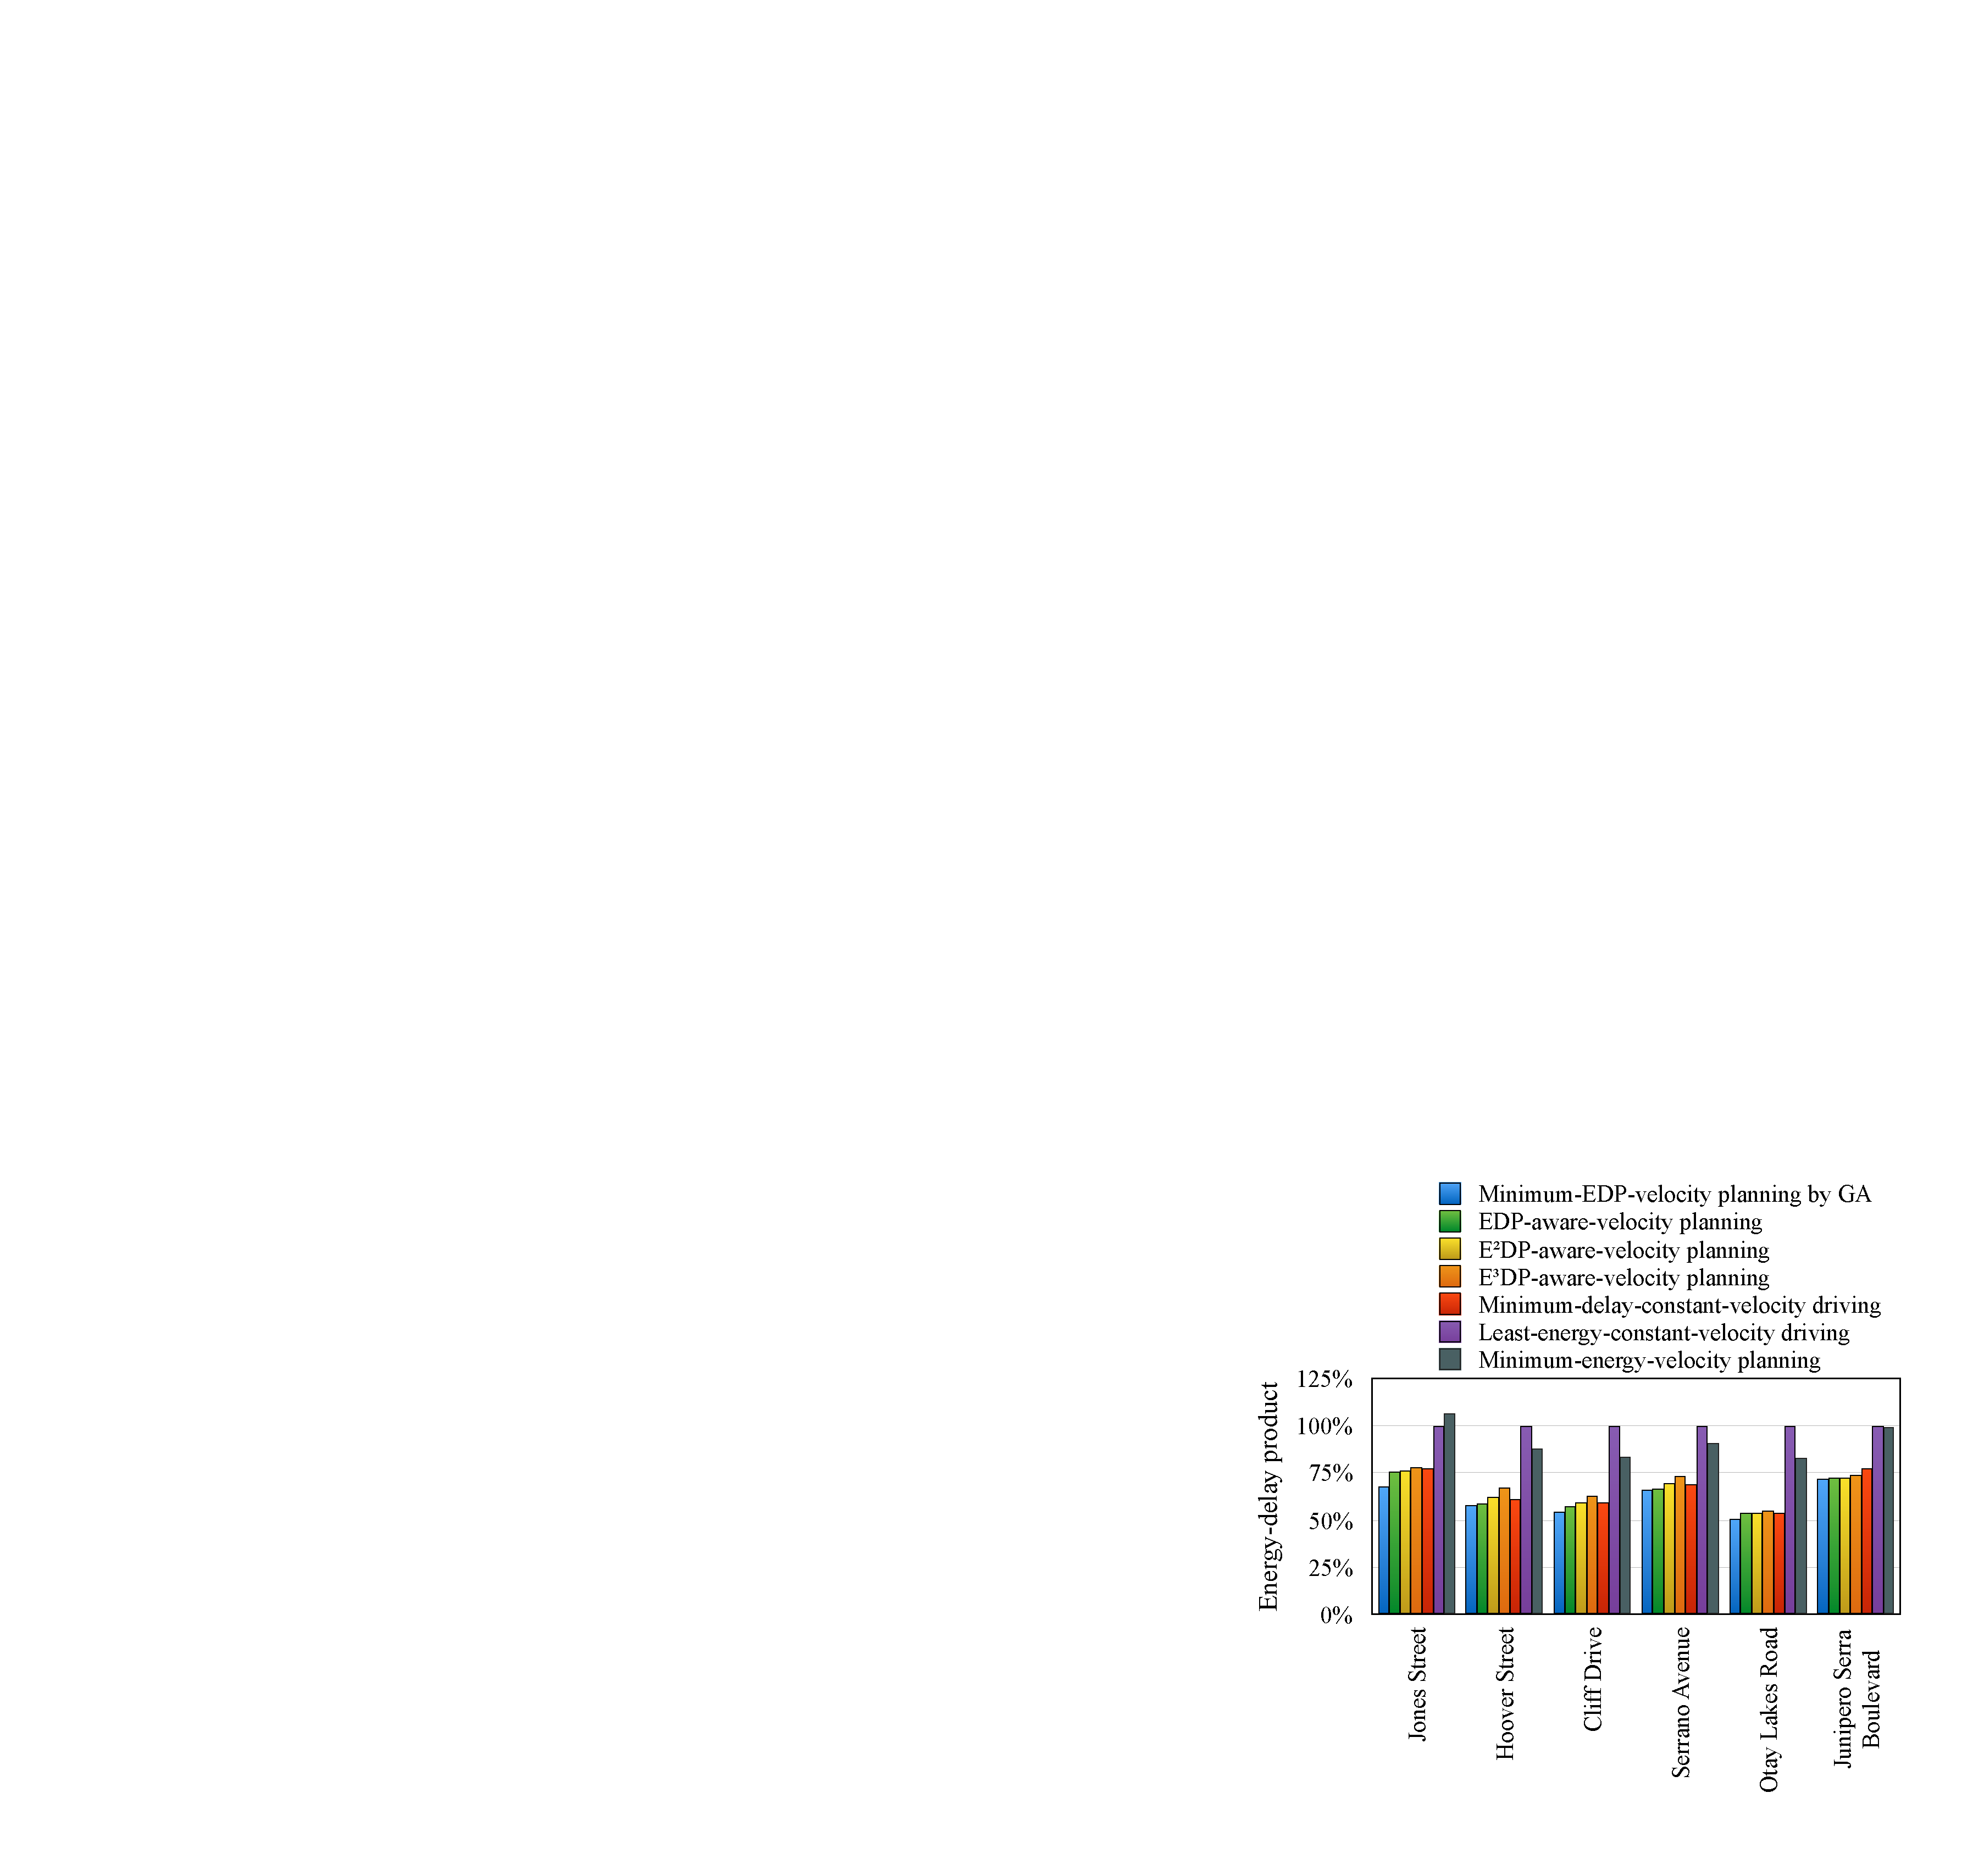
\includegraphics[width=0.6\hsize]{Figures/EDP_comp_bar.pdf}
\caption{\textcolor{red}{Comparison of $EDP$ for the proposed energy-aware-velocity planning methods.}}
\label{fig:EDP_bar}
\end{figure} 

\end{description}
\newpage
~

%%%%%%%%%%%%%%%%%%%%%%%%%%%%
\textbf{[REVIEWER 2]}
%%%%%%%%%%%%%%%%%%%%%%%%%%%%
\begin{description}

\item [R2-C1] The paper claims that the proposed BEV power model is more accurate than those in the literature. While the results in Section V demonstrate the benefits of the proposed model and in some way indirectly show its accuracy, it would be good to have a direct comparison of model accuracy between the proposed model and those in literature, e.g., based on simulations as in Fig. 1. 

\item [R2-A1] We appreciate the reviewers in that we can more efficiently deliver our technical contributions with a clearer evidence from the valuable comment. Reviewer 1 also questioned the BEV power model validation, and we added this contents in Section III-A on Page 3. The proposed EV power model well matches with the range-speed measurement  data provided by [32], [33], [34], [35], [36]. Please find the detailed answer with R1-A2: the answer (response) to the second comment of Reviewer 1.

\item [R2-C2] It would be good to have more discussion on the assumptions of the approach and the experiments, e.g., how much can the velocity be changed in practical scenarios without impeding traffic and causing unsafe situations (also depending on the road conditions and whether it is urban or rural environment I suppose). Currently, there only seems to be one constraint on not slower than 10 km/h. 

\item [R2-A2] In this paper, we assume the driving optimization is from a traffic signal to the next traffic signal or a stop sign to a stop sign, without considering an unexpected interrupt. However, it is not difficult to consider random interrupt by the use of an online recomputation whenever an interrupt occurs, but this may be off from the primary contribution of this paper. 

Nevertheless, give a lot of weight to the reviewer’s comment how the velocity is changed by the result of the proposed optimization. So, we put an extended time of effort to extensively analyze the velocity and acceleration change.

Of course, the least-energy-constant-velocity driving results in the least velocity and acceleration change, and thus it provides the maximum predictability and comfort. Compared with the least-energy-constant-velocity driving, the proposed methods, which are aware of $EDP$, $E^2DP$ and $E^3DP$, keep changing the velocity by the road slope change and thus may impede traffic as the reviewer pointed out. It is unlikely to incur dangerous situations, but harsh braking and fast deceleration may cause uncomfortness of passengers and potentially disturb safety assurance. In the revised manuscript, we add new analysis of the baseline and proposed methods ($EDP$, $E^2DP$ and $E^3DP$) about the velocity and acceleration change. The newly added analysis is a histogram analysis of velocity and acceleration. We quantize the velocity and acceleration values and make a histogram as shown in Fig. 11. Thanks to the reviewer’s comment, we had a chance to deeply look into the histogram analysis and revised the driving condition constraints. 

%We previously constrained that the EV should not drive too slow to avoid bothering traffic with the minimum speed of a 10 km/h. However, such velocity constraint is not realistic even in a city driving as the reviewer pointed out. We do agree on that more realistic minimum speed constraint is desirable, and thus we revised the constraint from 10 km/h to 25 km/h. Even with the new minimum speed constraint, we exhibit the same amount of gains with the proposed methods. After carefully analyzing the acceleration histogram, in this revised version of the manuscript, we newly enforce the minimum acceleration not lower than 1.0 $m/s^2$ when the EV starts from a stop sign or a traffic light until the velocity reaches to 25 km/h not too bother traffic flow. If the EV accelerates at a  1.0 $m/s^2$, it would take 15 seconds to reach a 25 km/h speed. The previous version of the manuscript used the maximum acceleration limited by the motor torque: a 4.7 $m/s^2$ on a flat road. However, such a fast acceleration negatively affects to the  power consumption as well as passenger comfortness. The revised version of the manuscript limits the maximum acceleration to 1.7 $m/s^2$ as shown in Fig. 13(b), which is the same as the maximum acceleration of compact cars designed to be primarily used in urban areas (15 seconds of 0-to-100 km/h time.)

Fig.~\ref{fig:histogram}(a) and (b) show two histograms of the driving schemes in Fig.~\ref{fig:EDP_aware_velocity_planning}, which do not have velocity and acceleration constraints. We avoid a cruising velocity lower than 25 km/h and an acceleration higher than 2.0 $\rm{m^2}/s$ in this paper without loss of generality. The  acceleration of 2.0 $m/s^2$ is the same as the maximum acceleration of compact cars designed to be used primarily used in urban areas (13 seconds of 0 to 100 km/h time).\\
Fig.~\ref{fig:histogram}(c) and (d) shows the velocity and acceleration histograms with the constraints. Once we run the DP for the first time without constraints, we analyze the histogram, adaptively determine the minimum cruising velocity and maximum acceleration constraints, and run DP again. We keep the same constraints for online recomputation whenever unexpected interrupts occurs.\\
We also enforce the minimum acceleration not lower than 1.0 $m/s^2$ when the EV starts from a stop sign or a traffic light until the velocity reaches to the minimum cruising velocity not to bother traffic flow. The acceleration of a 1.0 $m/s^2$ exhibits 6 second delay to reach 25 km/h. The maximum speed is bounded by the speed limit of each road benchmark.


\uline{We added Section IV-F on Page 8 is as follows:}\\
\textcolor{red}{Like the minimum-energy-velocity-planning, $E^2DP$- and $E^3DP$-aware-velocity planning methods may result in a too low cruising velocity, which bothers traffic as well as extends the driving time too much, and a too high acceleration may cause passenger discomfort. We add the velocity and acceleration constraints after first time running the DP. \\
We quantize the velocity and acceleration values and make a histogram to analyze population of velocity and acceleration for the proposed energy-aware-velocity planning methods. Fig.~\ref{fig:histogram}(a) and (b) show two histograms of the driving schemes in Fig.~\ref{fig:EDP_aware_velocity_planning}, which do not have velocity and acceleration constraints. We avoid a cruising velocity lower than 25 km/h and an acceleration higher than 2.0 $\rm{m^2}/s$ in this paper without loss of generality. The  acceleration of 2.0 $m/s^2$ is the same as the maximum acceleration of compact cars designed to be used primarily used in urban areas (13 seconds of 0 to 100 km/h time).\\
Fig.~\ref{fig:histogram}(c) and (d) shows the velocity and acceleration histograms with the constraints. Once we run the DP for the first time without constraints, we analyze the histogram, adaptively determine the minimum cruising velocity and maximum acceleration constraints, and run DP again. We keep the same constraints for online recomputation whenever unexpected interrupts occurs.} 

%% Description of driving constraints
\textcolor{red}{We also enforce the minimum acceleration not lower than 1.0 $m/s^2$ when the EV starts from a stop sign or a traffic light until the velocity reaches to the minimum cruising velocity not to bother traffic flow. The acceleration of a 1.0 $m/s^2$ exhibits 6 second delay to reach 25 km/h. The maximum speed is bounded by the speed limit of each road benchmark.}


\begin{figure}[h!]
\centering
 \renewcommand\thefigure{11}
	\begin{subfigure}{0.45\textwidth}
	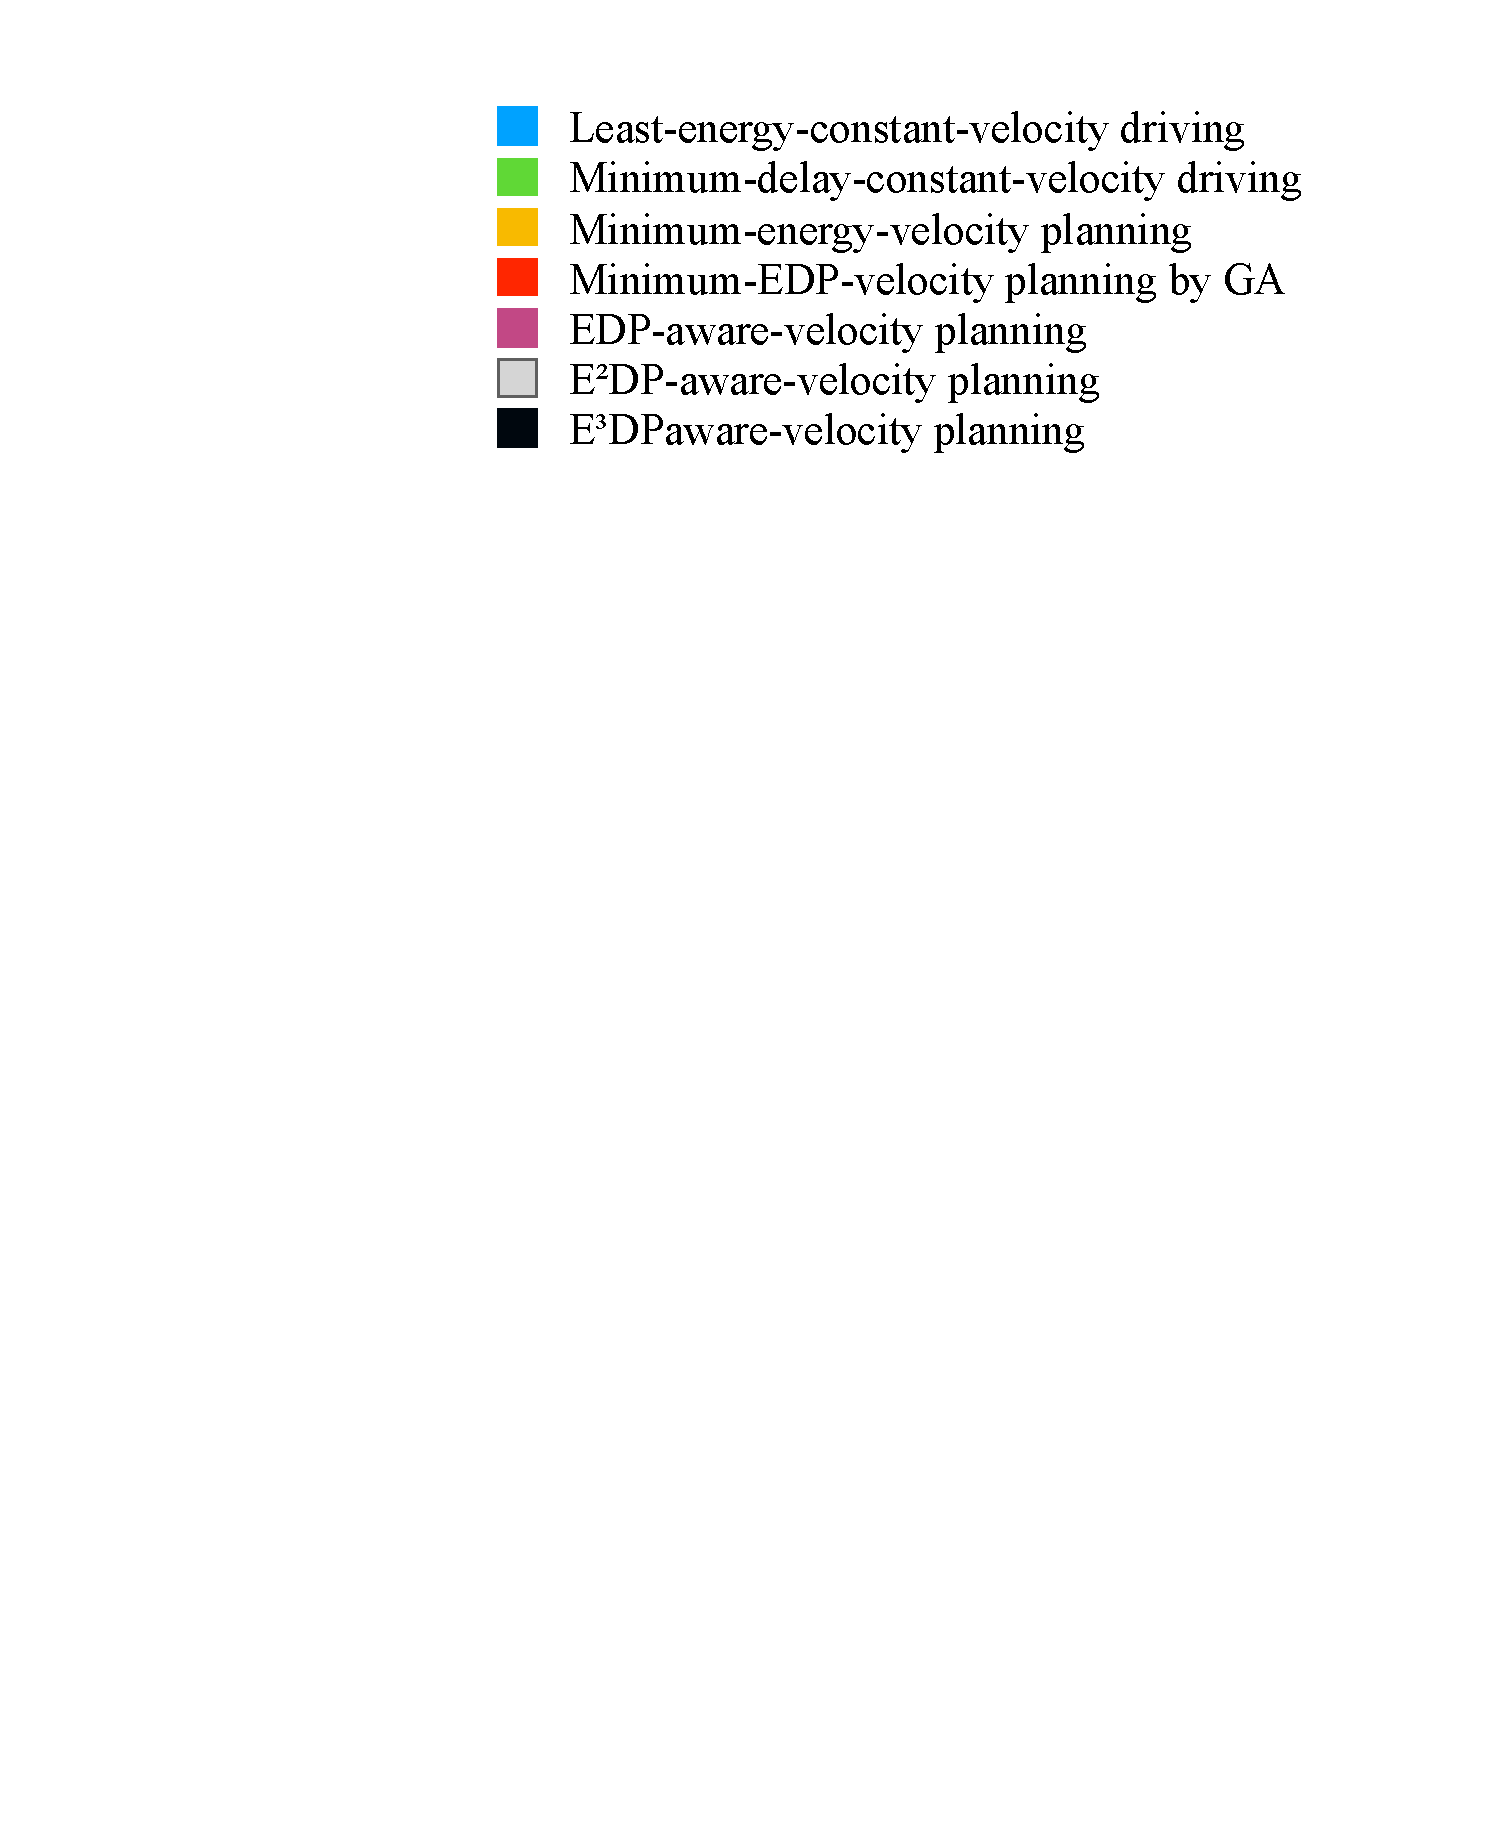
\includegraphics[width=\hsize]{Figures/Histogram_legend.pdf}
	\end{subfigure}
~\\
	\begin{subfigure}{0.45\textwidth}
	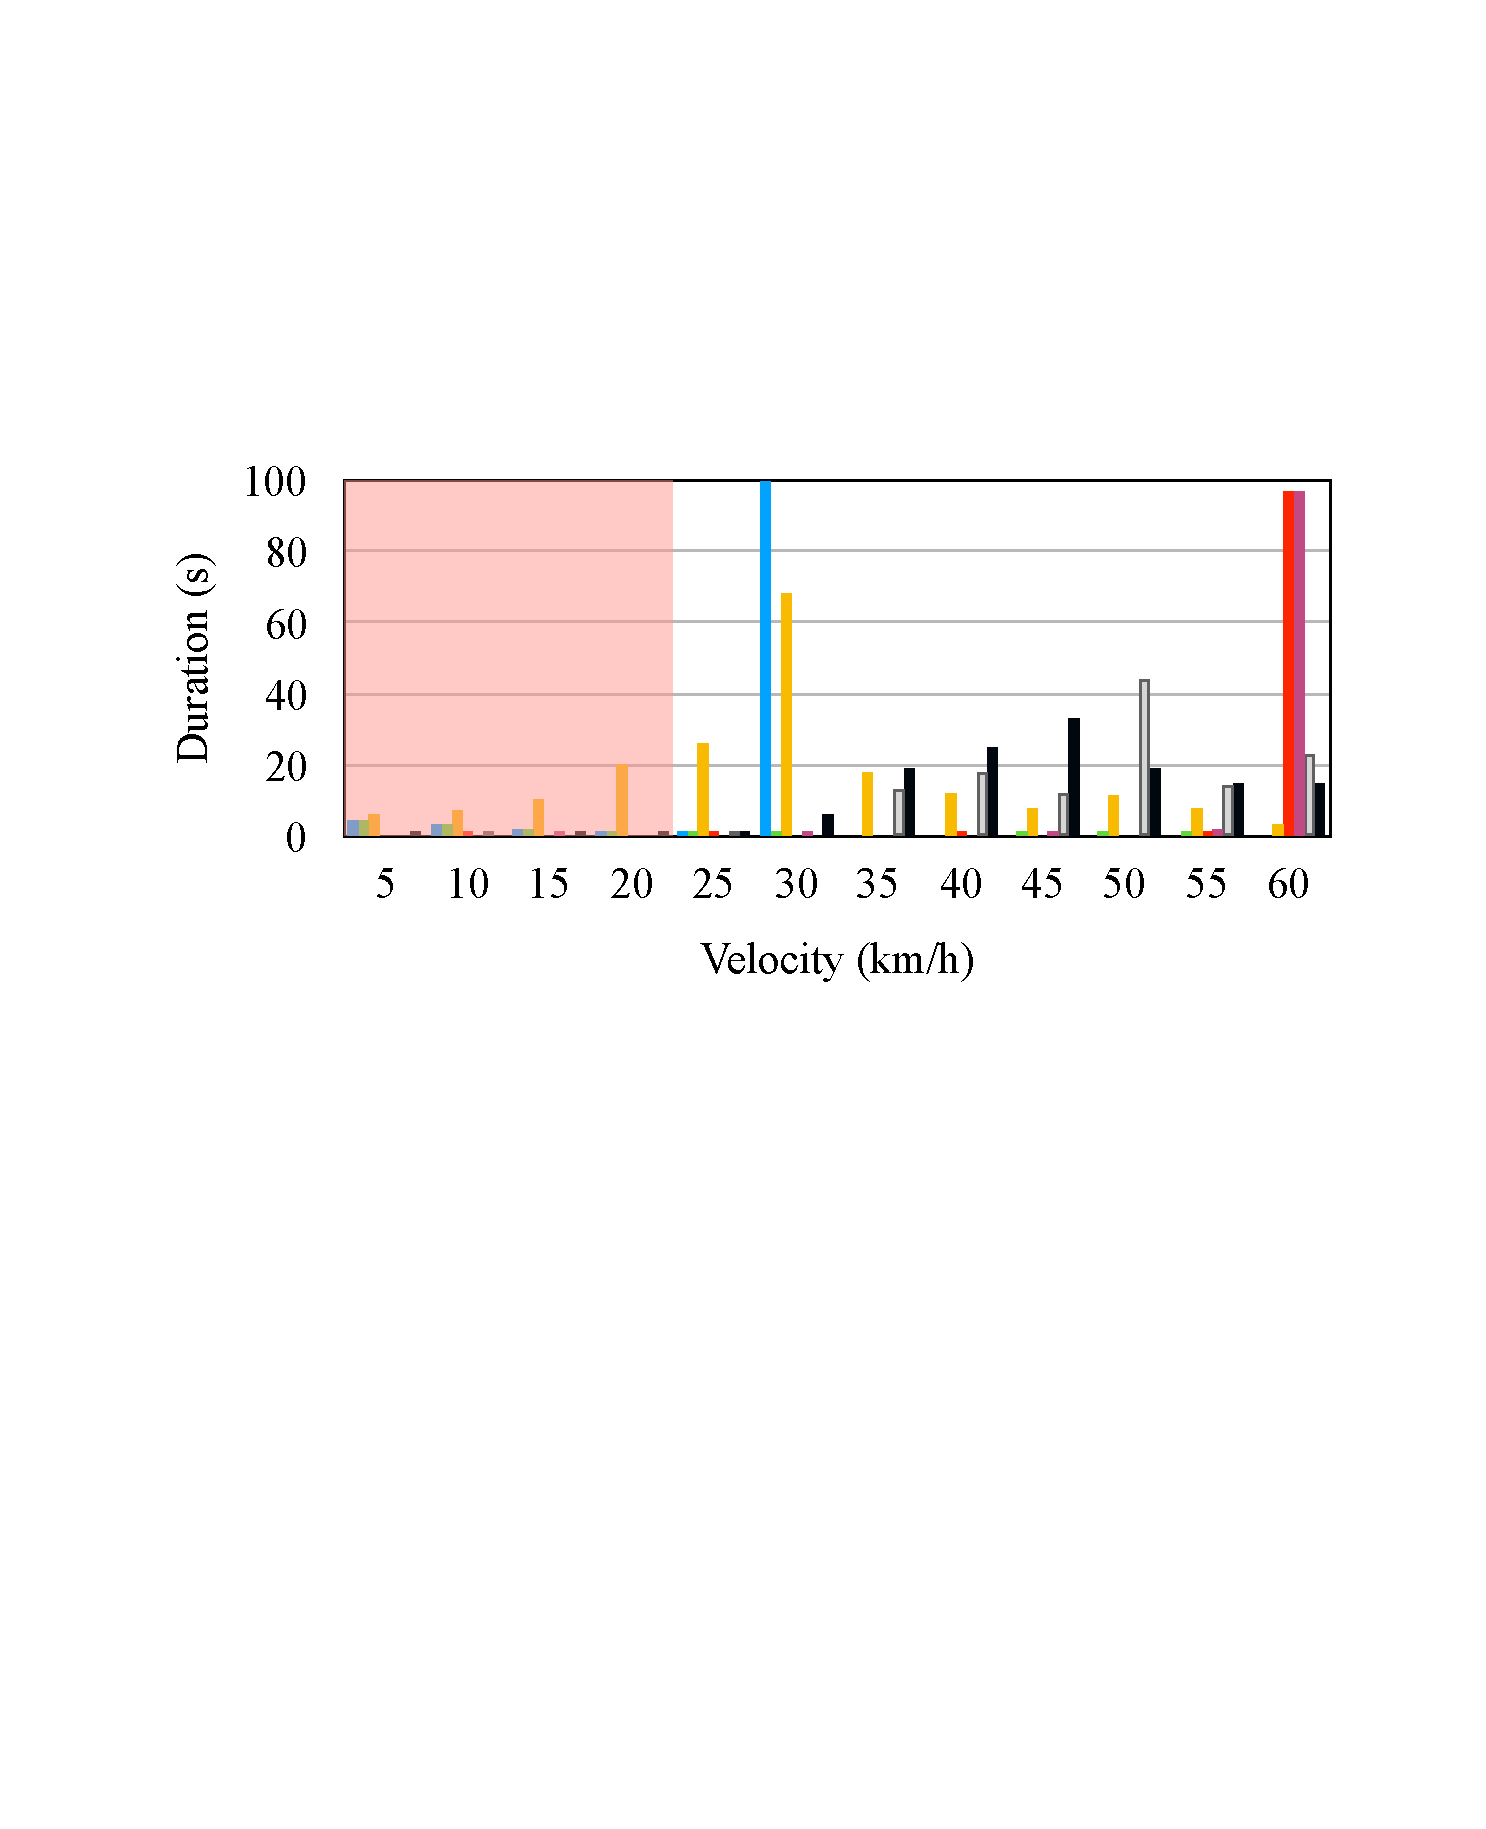
\includegraphics[width=\hsize]{Figures/Histogram_noconst_vel.pdf}
	\caption{A velocity histogram without constraints.}
	\label{fig:histogram_noconst_vel}
	\end{subfigure}
%~\\
	\begin{subfigure}{0.45\textwidth}
	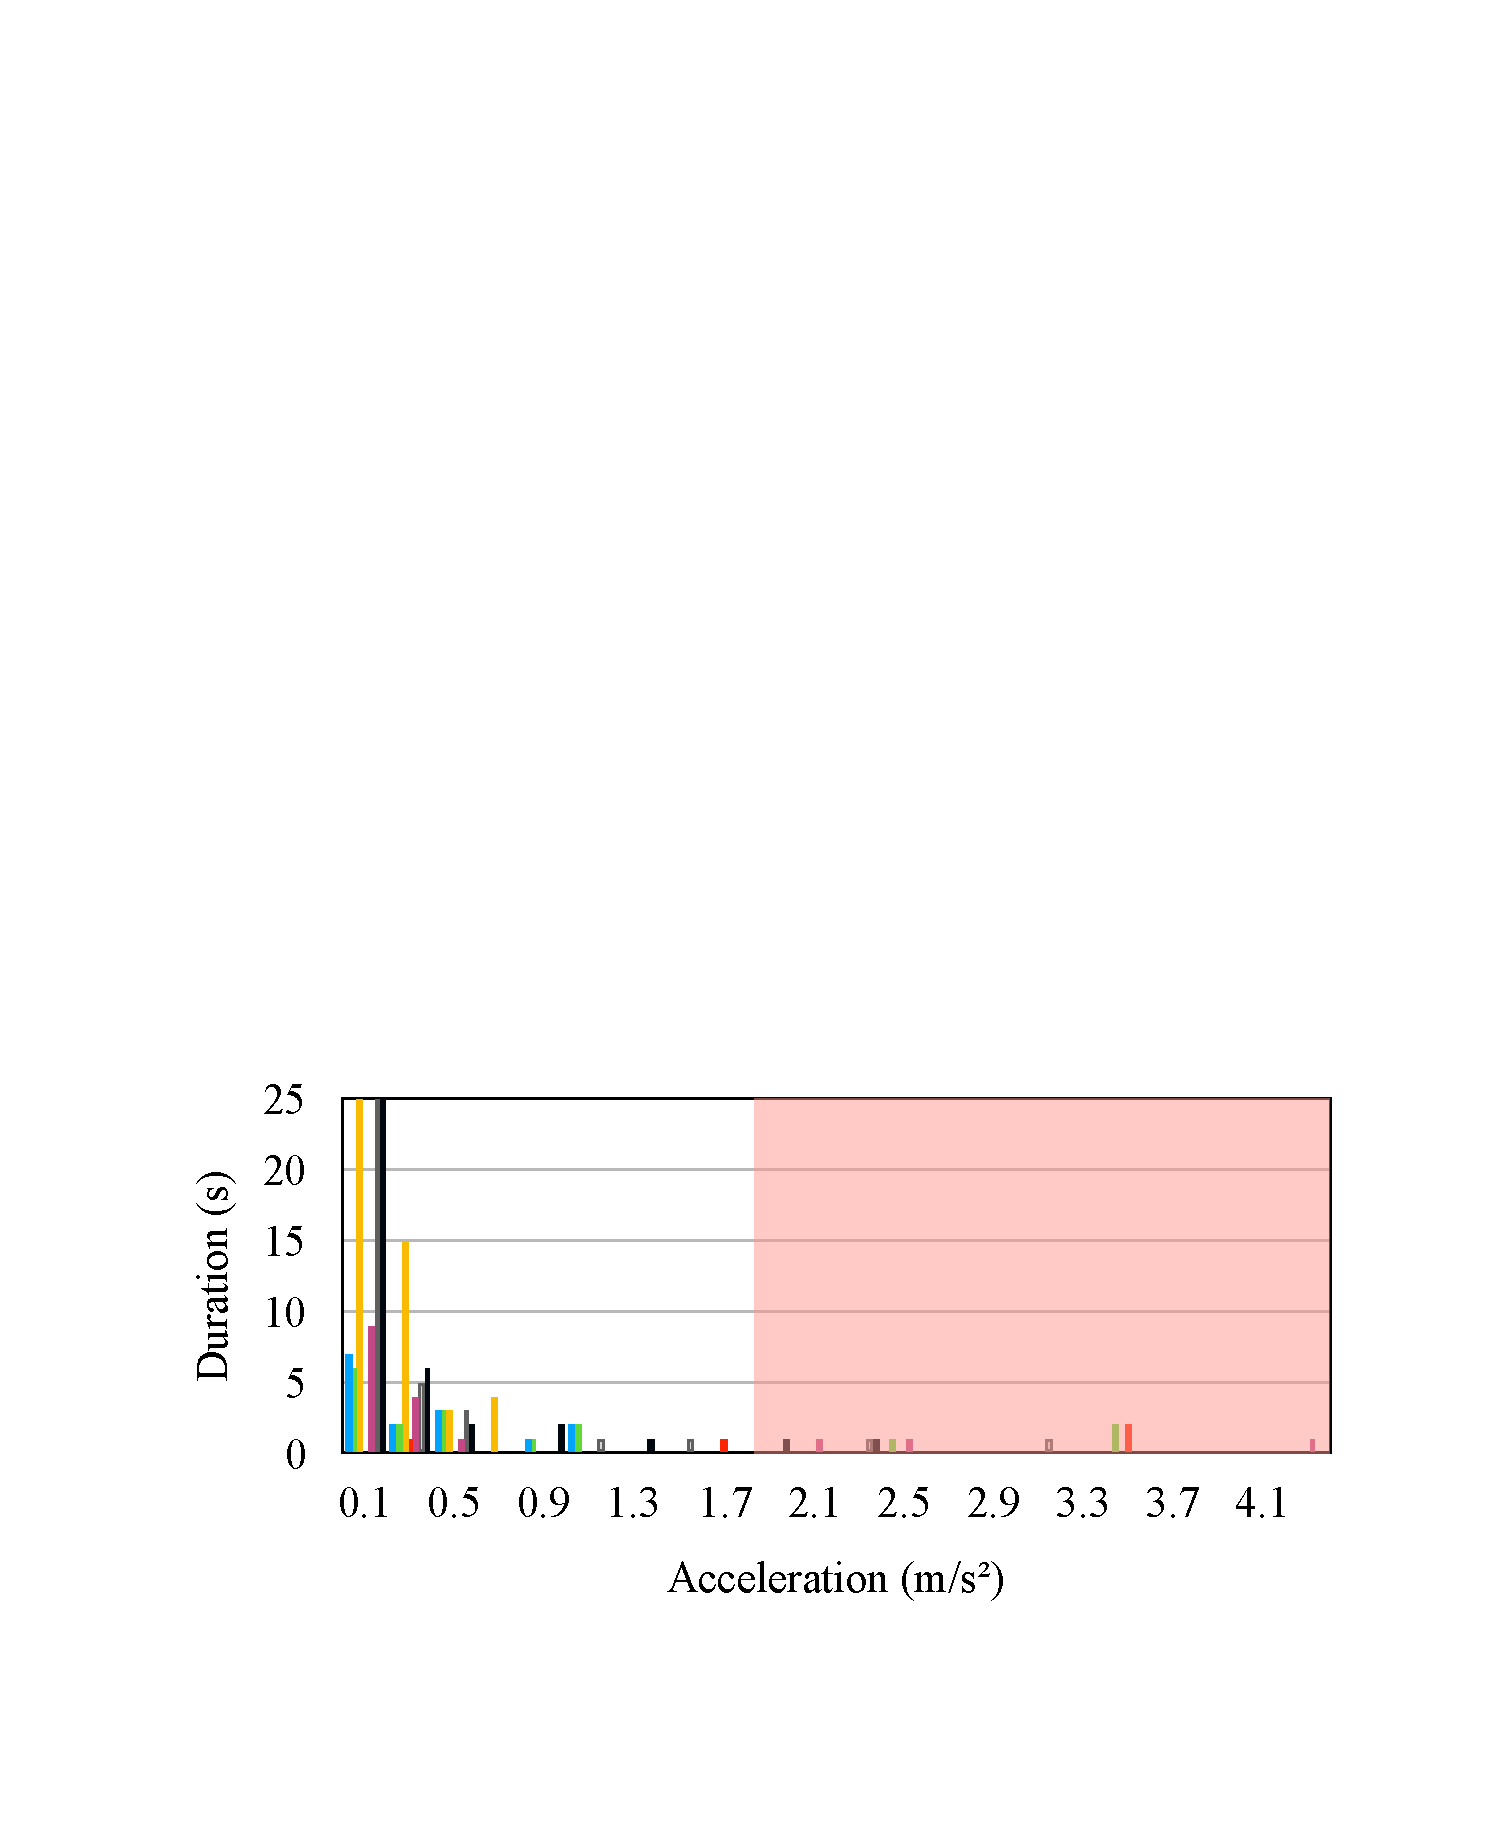
\includegraphics[width=\hsize]{Figures/Histogram_noconst_acc.pdf}
	\caption{An acceleration histogram without constraints.}
	\label{fig:histogram_noconst_acc}
	\end{subfigure}
%~
	\begin{subfigure}{0.45\textwidth}
	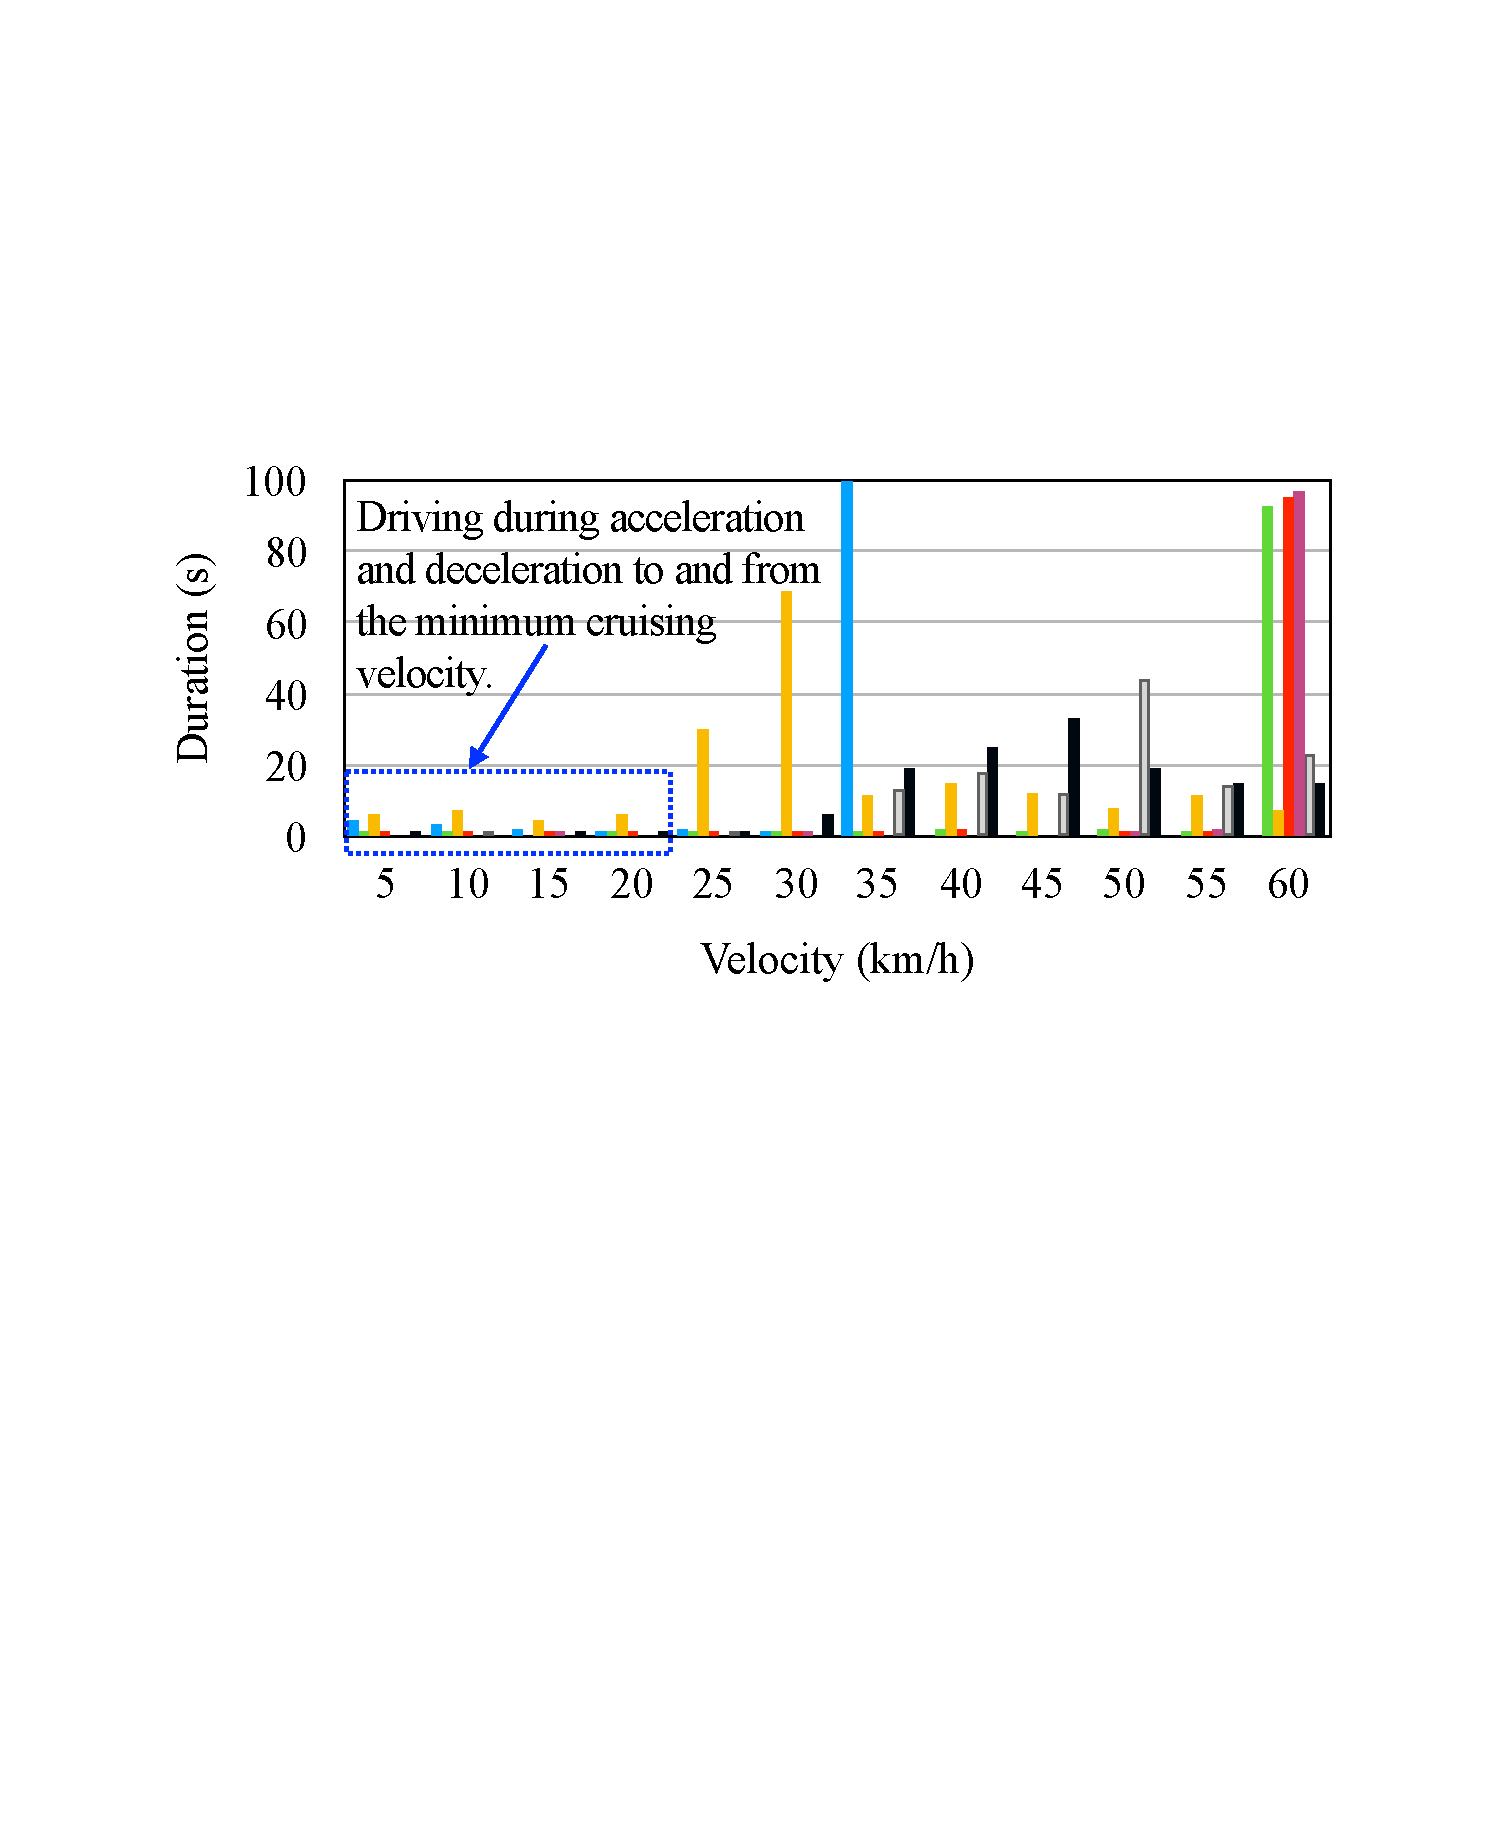
\includegraphics[width=\hsize]{Figures/Histogram_vel.pdf}
	\caption{A velocity histogram with constraints.}
	\label{fig:histogram_vel}
	\end{subfigure}
%~
	\begin{subfigure}{0.45\textwidth}
	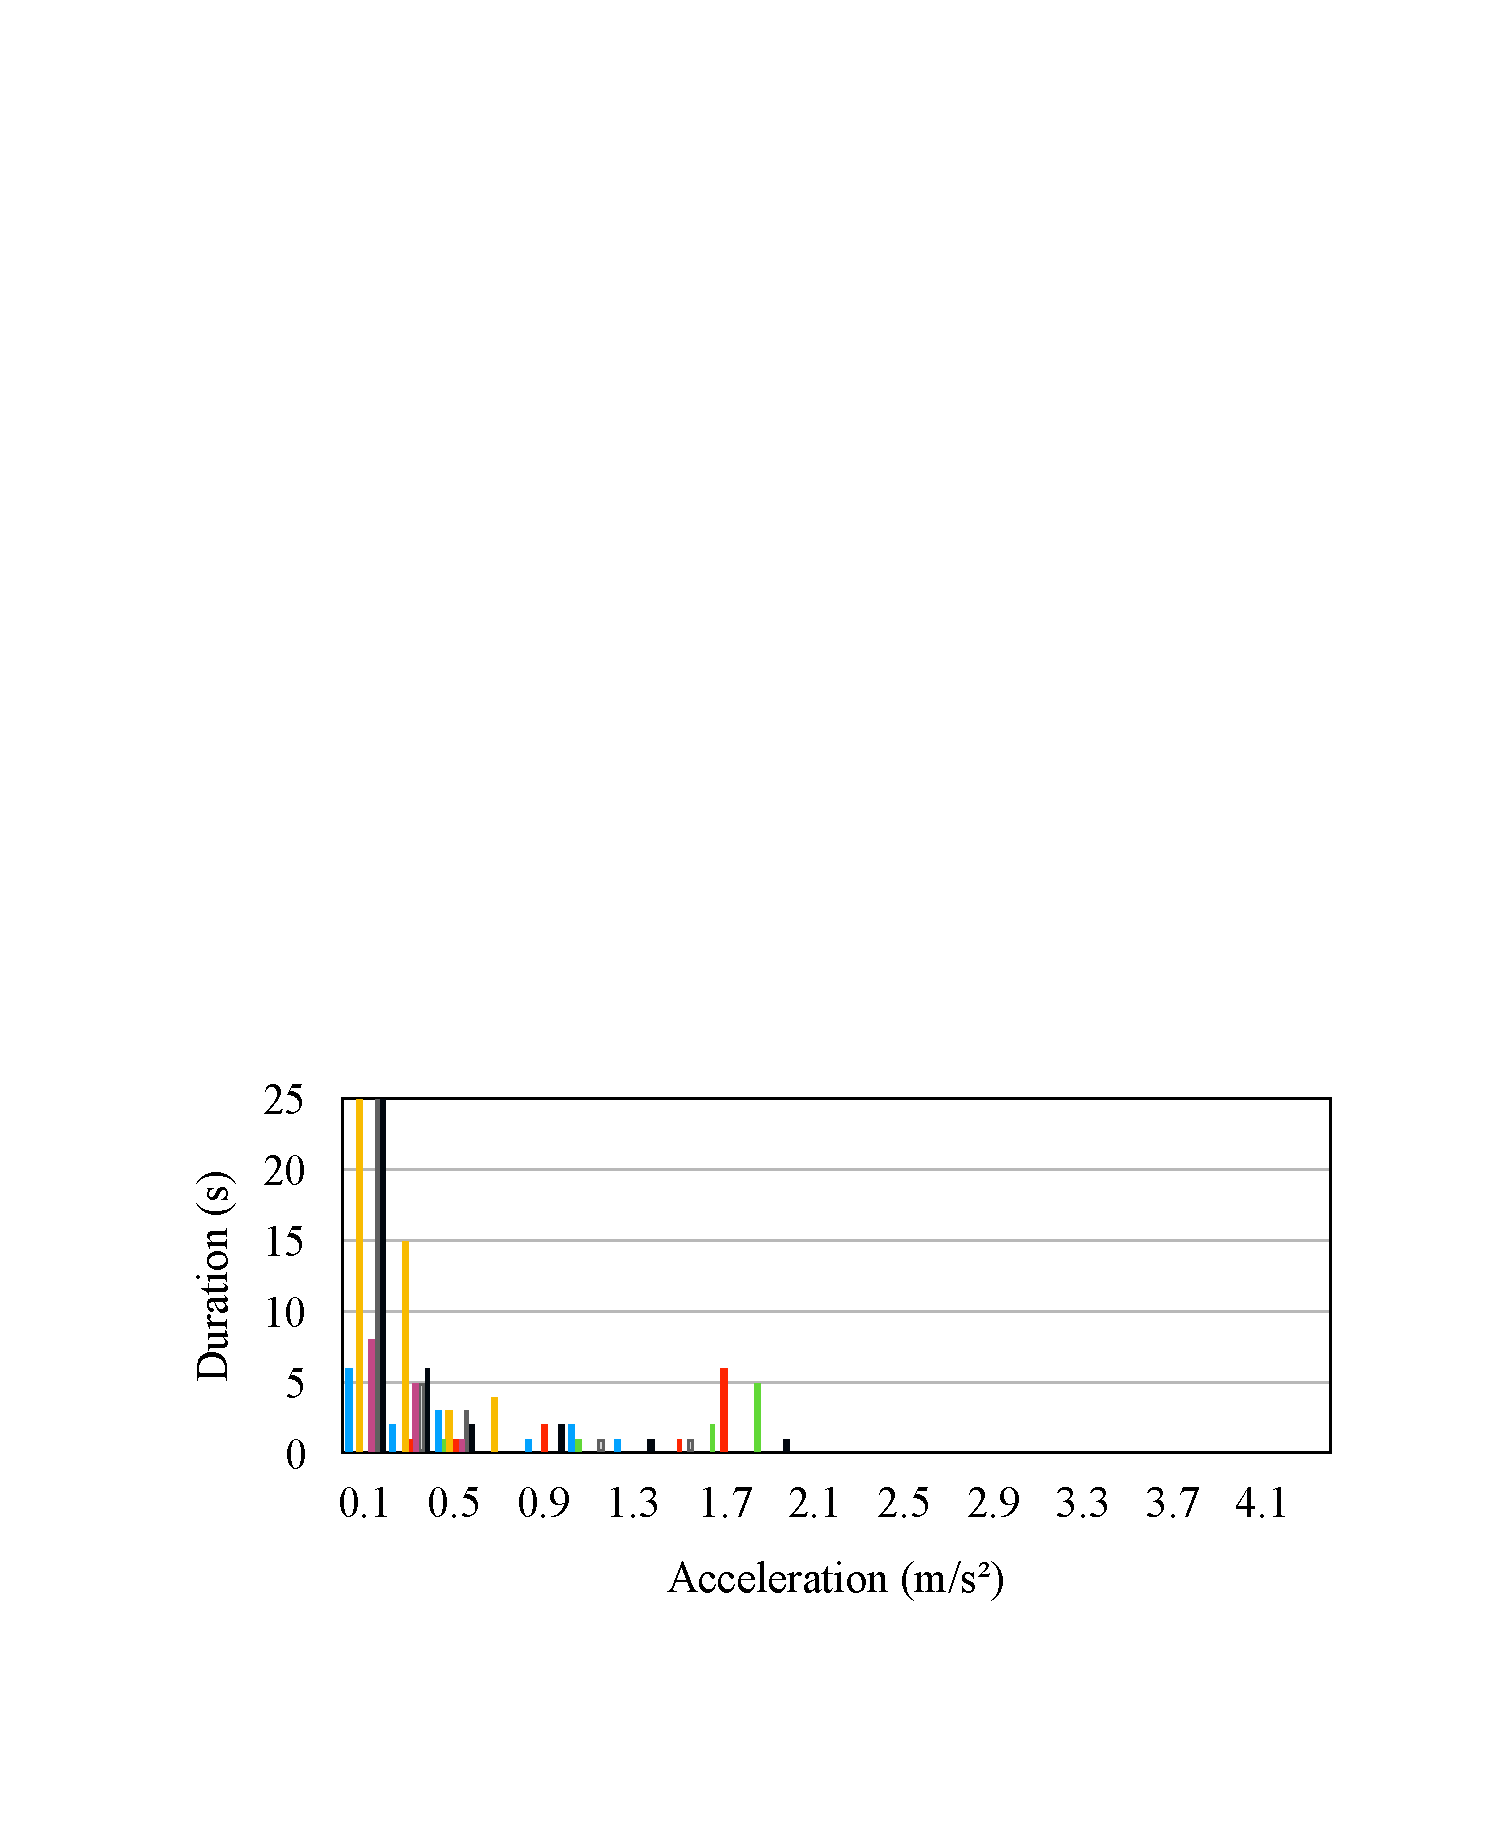
\includegraphics[width=\hsize]{Figures/Histogram_acc.pdf}
	\caption{An acceleration without constraints.}
	\label{fig:histogram_acc}
	\end{subfigure}
\caption{\textcolor{red}{Histograms of velocity and acceleration for the proposed energy-aware-velocity planning methods without an acceleration constraint (a) and (b) and with an acceleration constraint (c) and (d), respectively.}}
\label{fig:histogram}
\end{figure}

\item [R2-C3] Related to the last point, it would be good to have more discussion on the road benchmarks, e.g., how they are generated and how representative they are. The optimization results significantly depend on road slope. It would be good to use a variety of real road segments for testing.

\item [R2-A3] We appreciate the reviewer's comment. We replaced the previous synthetic road benchmarks with the real road benchmarks. We made six new real routes from various locations in California.  The first three roads are in cities. Jones Street in San Francisco and Hoover Street in Los Angeles are two representative city landscapes such as hills and flat roads, respectively, and Cliff Drive in Santa Barbara is a mixture of those. The second two roads are in mountain areas: Serrano Avenue in Anaheim Hills and Otay Lakes Road in San Ysidro Mountain in California. The last road is Junipero Serra Boulevard connecting San Fransisco and San Jose. The details of road data is summarized in Table~II, and Fig.~\ref{fig:bench_altitude}, which visualize the altitudes of the road benchmarks. We also revised all the associated contents with the new real road benchmarks. 

\begin{table} [h!]
%\caption{\textcolor{red}{Real road benchmarks.}}
\centering
\label{table:road_bench}
\begin{tabular}{|c|c|c|c|c|c|c|}  \hline
\multirow{2}{*}{Roads} 
				&Dist.		&\multicolumn{5}{|c|}{Road slope (\%)}  \\ \cline{3-7}
				&(m)		 	&Max.		&Min. 	&Mean		&RMS 	&Std.	\\ \hline
Jones St. 	&1257		&29.22		&-15.12	&4.97 		&12.31 	&11.27	\\ \hline
Hoover St. 	&1365		&8.45		&-7.44	&0.44		&1.08 	&0.99	\\ \hline
Cliff Dr. 	&1435		&4.77		&-2.75	&0.58		&1.77 	&1.67	\\ \hline
Serrano Ave.		&1797		&16.63		&-10.56	&1.14 		&4.10 	&3.94	\\ \hline
Otay Lakes Rd.		&1623		&6.80		&1.12	&3.24		&3.52 	&1.38	\\ \hline
Junipero Serra Blvd.	&1500		&7.46		&-5.48	&0.40		&2.72 	&2.70	\\ \hline
\end{tabular}
\end{table}


\begin{figure} [h!]	 %Figure 8.
\centering
\renewcommand\thefigure{8}
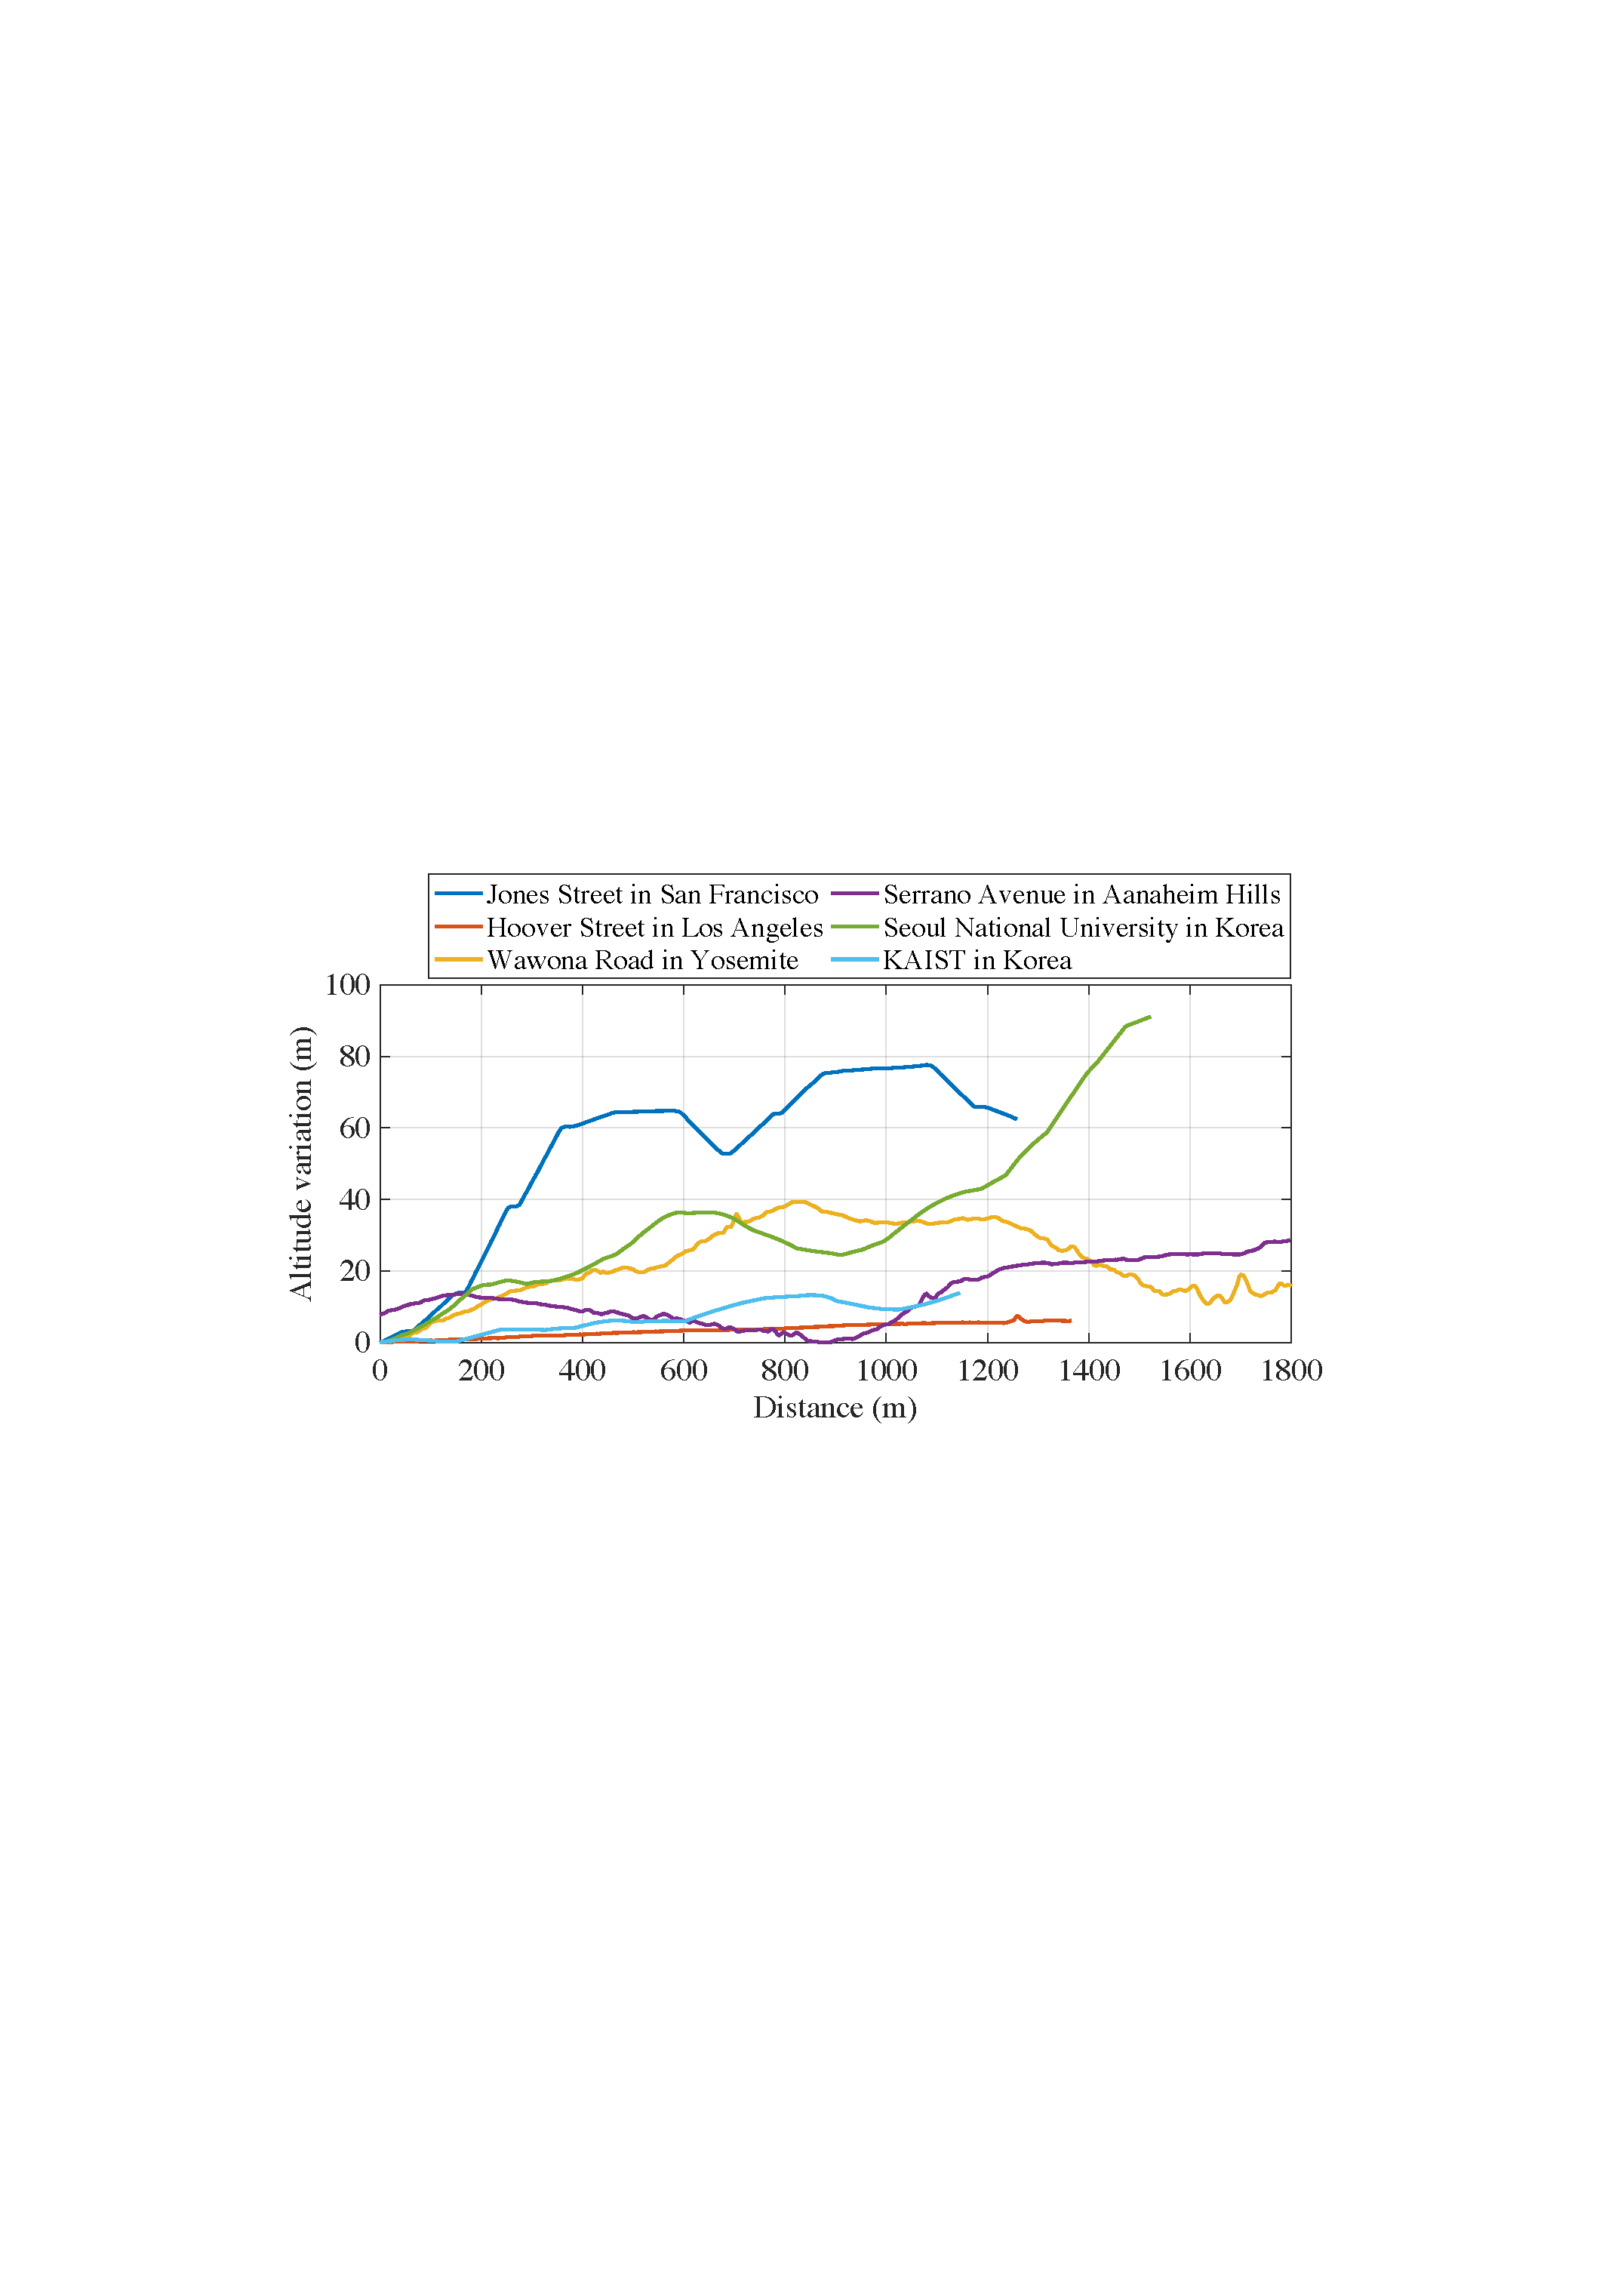
\includegraphics[width=0.7\hsize]{Figures/Benchmark_altitude.pdf}
\caption{\textcolor{red}{Altitude changes in the real road benchmarks.}}
\label{fig:bench_altitude}
\end{figure} 

%% Insert changes after manuscript is fixed

\item [R2-C4] The paper uses an online optimization approach. It is not very clear how often such optimization needs to be conducted and what its advantages are over offline approaches.

\item [R2-C5] We apologize a confusing statement such that ``This is absolutely not acceptable for online recomputation that can be caused by unexpected interrupts while driving,'' which sounds as if the proposed method is an online algorithm. Basically, we propose an offline driving optimization from a traffic signal to the next traffic signal or  a stop sign to a stop sign. Therefore, we assume that the driving optimization is done in advance before we drive the route.

However, we still offer online ``recomputation,'' which can produce a new solution in a reasonable amount of time if an unexpected interrupt occurs. For example, if a vehicle accident occurs, a GPS navigator may perform rerouting to detour the accident area. The proposed velocity planning should be ``recomputed'' for the modified route. After detouring, the new route will be merged to the original route, and we can still reuse the previously computed  velocity planning for the rest of travel. While the proposed methods can perform such online ``recomputation,'' the previous method that uses ADVISOR in the inner loop can hardly meet such requirement. 

\uline{We add the eighth paragraph in III-A on Page 3 as follows:}\\
\textcolor{red}{The proposed methods allows us to produce an updated solution in a reasonable amount of time if an unexpected interrupt occurs. For example, if a vehicle accident occurs, a GPS navigator may perform rerouting to detour the accident area. The proposed velocity planning should be ``recomputed'' for the modified route. After detouring, the new route will be merged to the original route, and we can still reuse the previously computed  velocity planning for the rest of travel. While the proposed methods can perform such online ``recomputation,'' the previous method that uses ADVISOR in the inner loop can hardly meet such requirement.}

\item [R2-C5] The baseline for comparison is the least-energy-constant-velocity scheme. As the optimal velocity significantly depends on road slope, such scheme is obviously sub-optimal. It would be interesting to see how the proposed method compares with a simple extension of least-energy-constant-velocity, where a constant velocity is calculated for each segment with the same slope.

\item [R2-A5] We appreciate the reviewer's suggestion. Review 1 also questioned the optimality of the proposed methods. Please  refer R1-A3. 

In addition, the reviewer suggested a ``segmented-least-energy-constant-velocity planning.'' Such extension may provide significant benefit to reduce the computation time because the least-energy-constant velocity for each slope is precalculated and stored in lookup table. 
However, the segmented-least-energy-constant-velocity planning have two major shortcomings. First, if the segment size is not small enough, there can a sudden acceleration or a deceleration when entering to a new segment if the road slop change is large. A sudden acceleration or deceleration certainly degrades the energy gain and passenger comfortness. Second, the segmented-least-energy-constant-velocity planning cannot find the globally optimal solution. As for a counterexample, the optimal minimum-energy-velocity planning (from DP) should increases  the speed before entering an uphill. This results in less energy consumption compared with the segmented-least-energy-constant-velocity driving at the top elevation (and the summit is the final destination.)  

\item [R2-C6] The paper is easy to follow. There are some minor issues/typos. For instance,
\begin{itemize}
\item Abstract, ``… from the vehicle dynamics, … , and consideration of regenerative braking.'' -> ``with the consideration of vehicle dynamics, … , and regenerative braking.''
\item Abstract, ``… (or at each time instant.) The major …'' -> ``… (or at each time instant). The major …''.
\item Page 1, column 2, ``but higher daily …'' -> `` but also higher daily…''.
\item Page 1, column 2, ``weight not to degrade …'' -> ``weight, and not to degrade…''.
\item Page 1, column 2, ``Such conventional ways … ownership.” -> ``These conventional ways of extending EV range may have a negative impact on the cost of ownership.”
\item Page 1, column 2, ``difference between that of ICEV” -> “differences from that of ICEV”.
\item Page 2, column 1, ``ICEVS” -> “ICEVs”.
\item Page 3, column 1, ``a sort of a fast vehicle simulator …” -> “a fast simulator”.
\item Page 3, column 2, ``demonstrates s …” -> “demonstrates …”.
\item Page 5, column 2, ``As total number of steps …” -> “As the total number of steps …”.
\item Page 5, column 2, ``total number of nodes and edges …” -> “the total number of nodes and edges …”.
\item Page 5, column 2, ``a distance” -> “the distance”.
\item Page 5, column 2, ``a power consumption” -> “the power consumption”.
\item Page 7, column 1, ``due unexpected interrupts.” -> “due to unexpected interrupts.”
\item Conclusion, ``legacy system-level …”. “classic” might be a better word than “legacy”.
\item Conclusion, ``a tight deadline constraint.” -> “a tight energy constraint?”.
\end{itemize}

\item [R2-A6] We sincerely appreciate such kind comments, and we also apologize typos. Thank you for helping us improve the revised  manuscript. We made all the corrections accordingly. 
\end{description}

~
\newpage

%%%%%%%%%%%%%%%%%%%%%%%%%%%%
\textbf{[REVIEWER 3]}
%%%%%%%%%%%%%%%%%%%%%%%%%%%%
\begin{description}

\item [R3-C1] The minimum energy velocity planning is effective. However, can you discuss how to address when the battery capacity decreases over time? How would your planning considers it?

\item [R3-A1] We assume the following three cases to correctly understand  the reviewer's intention about ``battery capacity decrease.''

\textbf{1) If the reviewer asked the battery voltage droop by the state of charge decrease:}

Lithium-Ion batteries exhibit a large output voltage difference by the state of charge. However, EVs are designed to produce the maximum motor torque throughout  the entire voltage range between the fully charged and fully depleted battery states. When the battery voltage drops according to the state of charge, the PWM controller increases the duty ratio to maintain the same effective output current. The same maximum motor torque is produced even when the battery is about to be fully discharged.

\textbf{2) If the reviewer asked the battery state of charge itself:}

The proposed  algorithms are already (virtually) globally optimal in terms of energy consumption meeting the other constraints (please refer R1-A3 for the optimality of the proposed methods). Therefore, there may not be a more beneficial planning considering the battery state of charge. In reality, the battery impedance is a function of the start of charge, the minimum energy consumption does not always imply the least discharge of the battery when it comes to a long-term high-C discharge. However, most real EV driving situations are not  long-term high-C discharge applications, and thus there may not be appreciable gain from the battery state of charge consideration.

\textbf{3) If the reviewer asked ``capacity fading," i.e., the battery capacity decrease by aging:}

The proposed algorithms are energy minimization meeting other constraints. So, the same optimality will be provided even for the aged batteries. 

\item [R3-C2] Three different energy-delay product metrics are given in the paper. Can you recommend which one would be the best practical scenarios?

\item [R3-A2] We appreciate the reviewer's insight to make the paper contribution clearer. Please refer R2-A2 for the histogram analysis of the speed and acceleration. We describe the details of he comparison of the proposed metrics in Section V-A. 

Of course, the least-energy-constant-velocity driving results in the least velocity and acceleration change, and thus it provides the maximum predictability and comfort. In the revised manuscript, we added new analysis of the baseline and proposed methods ($EDP$, $E^2DP$ and $E^3DP$) about the velocity and acceleration change. The newly added analysis is a histogram analysis of velocity and acceleration, which backs up the following statements in the previous version of manuscript.

%%
The minimum-delay-constant-velocity driving guides to accelerate to speed limit of the road benchmark (64 km/h). For the EDP-aware-velocity planning, it is used when the deadline is the most important concern. Therefore, it is also guided to drive near speed limit. The $E^2DP$- and $E^3DP$-aware-velocity planning methods are used when the remaining battery state of charge is more concerned than the deadline. It is guided to drive at an energy-efficient speed along a road slope. Particularly, the $E^3DP$-aware-velocity planning method is used when the state of charge is more concerned, and the driver should find the nearby charging station. It is guided to decelerate to 35-50 km/h.


\item [R3-C3] There are some parameter setting without discussion. For example, is there any specific reason to choose 42km/h in one of your experiments?

\item [R3-A3] We perform a design space exploration (DSE) for all feasible vehicle velocities and the acceleration pairs. We obtain the minimum-energy velocity and the initial and final acceleration for a given road. The point at the minimum energy consumption per distance (Wh/km) represents the least-energy-constant-velocity driving. The least-energy-constant velocity is 37 km/h for the benchmark route in Fig. 10. We added this new content in the revised version of the manuscript. 

\uline{We modify the fourth paragraph in IV-D on Page 7 as follows:}\\
\textcolor{red}{
Fig.~10 visualizes a more detailed picture how each driving method behaves on Serrano Avenue, for example. 
The point at the minimum energy consumption per distance (Wh/km) represents the least-energy-constant-velocity driving. The least-energy-constant velocity is 37 km/h in this example, which is achieved by a design space exploration (DSE). The minimum-delay-constant velocity is determined by 64 km/h, which is the speed limit of Serrano Avenue.}

\item [R3-C4] Time complexity analysis of the proposed techniques should be discussed.

\item [R3-A4] We propose a heuristics method that uses DP for the minimum-$EDP$, $E^2DP$ and $E^3DP$-velocity planning. DP solves the velocity planning in a polynomial time. The number of velocity states is a product of the number of selectable velocities in each distance $N$ and the number of steps to the endpoint $M$ as mentioned in Section IV-B. Also, the number of calculation to get the optimal velocity planning until the distance is $M$. Therefore, the complexity is $O(NM^2)$ for the minimum-energy-velocity planning and the proposed $EDP$-, $E^2DP$- and $E^3DP$-aware-velocity planning. We added this new content in the revised version of the manuscript. 
 
\uline{We add the sixth paragraph in IV-E on Page 8 as follows:}\\
\textcolor{red}{DP solves the velocity planning in a polynomial time. The number of velocity states is a product of the number of selectable velocities in each distance $N$ and the number of steps to the endpoint $M$ as mentioned in Section IV-B. Also, the number of calculation to get the optimal velocity planning until the distance is $M$. Therefore, the complexity is $O(NM^2)$ for the minimum-energy-velocity planning and the proposed $EDP$-, $E^2DP$- and $E^3DP$-aware-velocity planning.} 

\item [R3-C5] Is the vehicle used in your experiment general enough? Can you discuss the difference between the vehicle used in your experiment and those practical vehicles?

\item [R3-A5] In this paper, we use a model of Chevrolet Bolt, which has been produced since November 2016. Total 26,000 units have been  delivered, and Bolt is positioned as the third best-selling EV in the United States. We added this new content in the revised version of the manuscript. 

Reviewer 1 also questioned the BEV power model validation, and we added this contents in Section III-A on Page 3. The proposed EV power model well matches with the range-speed measurement data provided by [32], [33], [34], [35], [36]. Please find the detailed answer with R1-A2: the answer (response) to the second comment of Reviewer 1. 

\uline{We modify the nineth paragraph in III-A on Page 3 as follows:}\\
We choose Chevrolet Bolt (1,616 kg curb weight) for the target vehicle, but our method does not restrict a particular type of vehicles. \textcolor{red}{Chevrolet Bolt has been produced since November 2016. Total 26,000 cars have been  delivered, and Bolt is positioned as the third best-selling EV in the United States.} The top speed of Chevrolet Bolt is a 150 km/h. It is capable of achieving a 6.5 second 0--100 km/h time with a 150 kW electric permanent magnet motor~[30]. Chevrolet Bolt is equipped with a 350 V and 57.4 kWh Lithium-ion battery pack with 96-series and 3-parallel of 3.65 V cells~[31]. Chevrolet Bolt battery chemistry is Lithium Nickel Manganese Cobalt Oxide from LG. 

\end{description}
\end{document}



